\documentclass{article}


\usepackage{arxiv}

\usepackage[utf8]{inputenc} % allow utf-8 input
\usepackage[T1]{fontenc}    % use 8-bit T1 fonts
\usepackage{hyperref}       % hyperlinks
\usepackage{url}            % simple URL typesetting
\usepackage{booktabs}       % professional-quality tables
\usepackage{amsfonts}       % blackboard math symbols
\usepackage{nicefrac}       % compact symbols for 1/2, etc.
\usepackage{microtype}      % microtypography
\usepackage{lipsum}
\usepackage{graphicx}
\graphicspath{ {./images/} }

\usepackage{lmodern}%
\usepackage{textcomp}%
\usepackage{lastpage}%
% \usepackage[margin=0.5in]{geometry}%
\usepackage{float}%
\usepackage{xcolor}
\usepackage[export]{adjustbox}
\usepackage[numbers]{natbib}
\usepackage{listings}
\usepackage{minted}
\usemintedstyle{vs}
\usepackage{subfig}
\usepackage{multirow}

\renewcommand{\arraystretch}{1.5}



\title{Accelerated Atomistic Modelling of Aluminum Precipitates: A Case Study with Al-Cu}

\author{
 Daniel Marchand \\
  Institute of Materials Science \\
  École Polytechnique Fédérale de Lausanne \\
  CH-1015, Vaud, Switzerland \\
  \texttt{daniel.marchand@epfl.ch} \\
  %% examples of more authors
   \And
 Albert Glensk \\
  Institute of Mechanical Engineering \\
  École Polytechnique Fédérale de Lausanne \\
  CH-1015, Vaud, Switzerland \\
  \texttt{albert.glensk@epfl.ch} \\
  \And
 William Curtin \\
  Institute of Mechanical Engineering \\
  École Polytechnique Fédérale de Lausanne \\
  CH-1015, Vaud, Switzerland \\
  \texttt{william.curtin@epfl.ch} \\
  %% \AND
  %% Coauthor \\
  %% Affiliation \\
  %% Address \\
  %% \texttt{email} \\
  %% \And
  %% Coauthor \\
  %% Affiliation \\
  %% Address \\
  %% \texttt{email} \\
  %% \And
  %% Coauthor \\
  %% Affiliation \\
  %% Address \\
  %% \texttt{email} \\
}

\begin{document}
\maketitle
\begin{abstract}
Precipitates are fundamental to the strengthening of aluminum alloys, and understanding them is paramount for optimized processing.
Precipitates are highly complex, and their formation sequence, kinetics, and the resulting influence on mechanical properties must be studied at the atomic scale, particularly during early-stage nucleation and growth.
Atomistic modeling via Density Functional Theory (DFT) is well-established and has been successful for a wide variety of precipitates; however, it is extremely computationally expensive and typically limited to modeling relatively simple bulk properties. On the contrary, interatomic potentials are computationally affordable, yet tend to lack accuracy. A promising new method for modeling precipitates is through the use of interatomic Neural Network Potentials (NNPs), that have near-DFT accuracy without the massive cost. 
Here, we present a demonstration of NNPs for Al-Cu based-alloys, 
their $\theta''$ $\rightarrow$ $\theta'$ $\rightarrow$ $\theta$ precipitation sequence
being one of the oldest and most investigated in the field, providing a model system for comparison.
We demonstrate the high fidelity of the Al-Cu NNPs for predictions of intermetallic compound energetics, elasticity, dilute solid-solution binding, interfaces, generalized stacking fault energy surfaces, and anti-site defect energies.
We further show that our NNP can correctly the entropically-induced shift between $\theta'$ and $\theta$, 
\textcolor{red}{I AM TENTATIVELY PROPOSING A KMC SECTION SINCE ABHINAV'S RESULTS SEEM PROMISING} while with Kinetic Monte Carlo we show our NNP can model early-stage GP \textcolor{red}{AND GP2?} zone formation.
This work points to a new and powerful approach for advancing the predictive understanding of Al alloys. 
\end{abstract}


% keywords can be removed
%\keywords{First keyword \and Second keyword \and More}


\section{Introduction}
Aluminum is one of the critical materials in the modern world.
Pure Aluminum is almost useless because of its low yield point\cite{Nie2014PhysicalAlloys}; defects are what give Aluminum its utility, its strength.
Precipitates are, arguably, the most essential, and most complex defects for understanding Aluminum's mechanical properties.
Heat is almost always needed to obtain the optimal type and size of precipitates, so much heat, that aluminum production is one of the largest energy-consumers of the planet\cite{Raabe2019StrategiesMetals}.
It is not trivial to predict the amount of heat needed, or even the concentration of elements to add, as the mechanical properties are the unique function of dozens of alloying elements and innumerable processing conditions.

Good atomic models are essential in the study of aluminum precipitates, firstly, because the initial formation of precipitates involves small clusters of atoms, too small to be viewed with ease in experiments.
Secondly, because the interactions between dislocations and small precipitates are discrete, and does not readily lend itself to continuum modeling.
The challenge is to find atomic models that are both accurate and fast.
Density Functional Theory (DFT) is very accurate, but incredibly slow modeling more than a few hundred atoms in DFT is exceptionally challenging\cite{Martin2004}.
Atomic potentials are fast, but often inaccurate, it is challenging to have atomic potentials model all of the properties relevant to precipitate formation, growth, and influence on mechanical properties.

Defects control the mechanical quality of aluminum alloys;
solutes and precipitates are the primary barriers to dislocation propagation.
Single solutes may attract or repel each other depending on their solute binding energies and form clusters with time.
Clusters, given enough time and enough heat, transform into precipitate structures within the matrix.
Precipitate stability depends on many factors\cite{Giofre2017}: bulk enthalpy, elastic strain, interface energy, and in some cases, such as $\theta'$ and $\theta$, precipitates can be very sensitive to entropic vibrations as well.
Then the resistance these precipitates give to incoming dislocations is highly dependant on their generalized stacking fault energy surface.
Finally, real alloys are complex, and often precipitates take on a non-stoichiometric form the propensity for this to happen is controlled by antisite and vacancy energies\cite{Kim2018}.
Therefore, a good potential should capture all these properties:
solute binding energies, formation enthalpies, atomic volumes, misfit volumes, elastic constants, interfacial energies, generalized stacking fault surfaces, and antisite and vacancy energies. 

In this work, we focus on Al-Cu as a case study for atomic modeling.
It has been well-studied for a long time\cite{Preston1938StructureAlloys}, thus making it nicely comparable for benchmarks.
Furthermore, it exhibits several properties that are challenging to model, notably the entropically-driven $\theta'$→ $\theta$ transformation \cite{Wolverton2001b}.

Apostol and Mishin created an Angular Dependent Potential (ADP) for Al-Cu systems.
In their work, they focused on modeling: formation energies, lattice constants, elastic constants, surface energies, and generalized stacking fault energies\cite{Apostol2011}.
The potential became very popular and was used in numerous studies of mechanical behavior of precipitates,
in studying solute and precipitate strengthening\cite{Singh2013AnAlloy}\cite{Esteban-Manzanares2019}\cite{Wu2020AtomisticAlloys}.
Work by Kobayashi et al. \cite{Kobayashi2017} studied Al-Mg-Si with Neural Network Potentials (NNPs), and they had found excellent results in modeling precipitate-relevant properties beyond what was possible with other potentials for that system.

Our goal in this work was to attempt to construct an NNP that would improve state of the art in precipitate modeling, where we use ADP a comparison.
We carefully, systematically examined all the atomic-level properties that would be relevant to precipitate modeling: solute/vacancy interactions, formation energies, elastic constants, interface energies, generalized stacking fault energies and the as-mentioned entropic stability of $\theta'$ over $\theta$ phase.

\section{Methodology}
\subsection{Atomic Structures}
\textcolor{red}{This paragraph risks overlapping with the introduction.
The section seems a bit strange now, like I"m just writing out a list}
We wished to study and include as many atomic structures relevant to precipitation as possible.
 Here we briefly outline the structures we considered in this study, with \textcolor{red}{further details in the relevant sections and the supplementary}.  
Firstly we needed a broad range of bulk Al-Cu compounds and made use of all those in the Open Quantum Materials Database \cite{Kirklin2015}.
Early-stage clustering was considered by looking at 2, 3, and 4 atom clusters of dilute Cu in Al. We also looked at a large number of 32 atom FCC supercells spanning all concentrations ratios of Al/Cu in units of 5\% 
with random atomic distortions to broaden the configuration space sampled.  For interfaces, we considered both the coherent and semicoherent interfaces of both $\theta''$ and $\theta'$.  We also considered surface energies,  stable and unstable stacking faults, solute-stacking fault interactions for pure Al and Cu.
We wanted valid elastic constants thermal and for all these structures, and made use of pymatgen\cite{Ong2013} and Phononpy\cite{Togo2015FirstScience} to generate the relevant deformations.
We also included GSF structures to model mechanical response to dislocations accurately. Finally, we considered
antisites and vacancies by swapping out elements of structures in the OQMD. A list of all categories of structures considered, and their number are in Table \ref{table:included_structures}.

\begin{table}[H]
\begin{tabular}{l|c}%
\hline%
Structure Category& Number Structures\\%
\hline%
Prior Work (Al only) &	555 \\
Phonons &	184 \\
Bulk and Elastic  &	2163 \\
Random FCC	& 990 \\
Binary Solutes & 	690 \\
Solute Stacking Fault &	54 \\
Stacking Faults &	111 \\
Surfaces &	87 \\
Interfaces &	8 \\
GSF ($\theta$ only)	 & 15 \\
\hline
Total &	4857 \\
\end{tabular}%
\caption{All structures considered for training. 24 $\theta''$ GSF structures and 230 Antisite structures were 
also looked at, but only for validation and not for training}
\label{table:included_structures}
\end{table}


\textcolor{red}{This paragraph probably needs to be moved elsewhere? 
Should I move other structure descriptions here?} The OQMD was the primary source of structures used when training and
testing the NNP across a broad range of Al-Cu compounds. $\theta$ and $\theta''$ were not in the OQMD, and we
included them as well manually for a total of 62 structures. Each of these structures was then fully relaxed, 
both in cell dimensions and atomic positions. Because we wished to avoid testing duplicates, only structures that retained the same symmetry group before and after relaxation were explicitly compared against the ADP and NNP
potentials (N=47). The elastic tensor was computed similarly to \cite{DeJong2015}, where a finite set of strains were
applied and fitted to the associated stresses. The pymatgen package\cite{Ong2013} determined the minimal number of
deformations required for each structure based on its symmetry, and only these were used. 
Unless stated otherwise, we computed formation energies using FCC Al and FCC Cu as the corresponding ground states. 

\subsection{NNP selection and Evaluation of Errors}
In this work, we generated NNPs using the methodology developed by Behler and Parrinello\cite{Behler2007}.
Here we only sketch out the essential basics of NNPs and refer the reader to the excellent tutorial review of Behler for further details \cite{Behler2015}. 


An NNP predicts the energy of an entire structure, by summing energies predicted on each atom within the structure: 
\begin{equation}
E^{structure} = \sum_i E^{atom}_i
\end{equation}
Each atomically-local energy, $E^{atom}_i$, is a nested hierarchical function of weighted layers across the neural network.
Where In our case, with two hidden layers, and 24 nodes per layer the functional form would be:
\begin{equation}
E^{atom}_i = f_3 \Large( b^3_1+\sum^{24}_{k=1}a^{2,3}_{k,1}\cdot f^2_k\Large(b^2_k+\sum^{24}_{j=1}a^{1,2}_{j,k}\cdot f^1_j \Large( b^1_j + \sum^{64}_{i=1} a^{0,1}_{i,j}\cdot G_i                 \Large)\Large)\Large) 
\end{equation}
Where $a^{q,p}_{z,w}$ is the weighting from node $z$ on layer $q$ to node $z$ on layer $w$, similarly $b^q_z$ is
the bias of node $z$ on layer $q$. $f_q$ is an activation function, in our work we used used the softplus function,
$\ln (1 + \mathrm{e}^x)$ for $f_1$ and $f_2$ and $f_3$ is the identity function. 
We used both radial and angular symmetry functions as  defined as follows:
\begin{equation}
G^{radial}_i = \sum^{N_{atom}}_{j=1}e^{-\eta(R_{ij}-R_{s})^2}\cdot f_c(R_{ij})
\end{equation}
\begin{equation}
G^{angular}_i = 2^{1-\zeta}\sum_{j\neq i}\sum_{k\neq i,j}\large[ (1+\lambda\cdot cos\theta_{ijk})^\zeta \cdot e^{-\eta(R^2_{ij}+R^2_{ik}+R^2_{jk})}\cdot f_c(R_{ij}) \cdot f_c(R_{jk}) \cdot f_c(R_{jk}) \large]
\end{equation}

Where $\eta$, $\zeta$ and $\lambda$ are the defining hyperparameters of a given symmetry function, $R_ij$ is 
the distance between two given atoms, is a cutoff function. 
We selected symmetry functions with the method of Imbalzano et al.\cite{Imbalzano2018}.
Firstly, we generated a dense grid of 1192 unique radial and angular symmetry functions.
We then performed a CUR decomposition and selected the 32 most descriptive Al-centered symmetry functions and the 32 most descriptive Cu-centered symmetry functions for a total of 64 symmetry functions.
The training of the NNP potentials was handled by the n2p2 library\cite{Singraber2019ParallelPotentials}\cite{Singraber2019Library-BasedPotentials}.
We used 10\% of the structures for testing and the remainder for training.
NNP weights were updated during the training using a fading memory Kalman filter.
The exact settings used are in the supplementary materials.
LAMMPS\cite{Plimpton1995} was used for running all calculations via the n2p2 interface. 

In this work, we trained several NNPs (N=40) to estimate expected errors. We selected the NNP with the lowest error for $C_{44}$ in aluminum to be the single representative example because of the importance and relative difficulty, as will be discussed later, of modeling $C_{44}$ correctly. All error bars center on the average of all trained NNPs and extends their standard deviation outwards. Thus, the representative NNP, i.e., the NNP with the closest $C_{44}$ to DFT, is not always close to the error bar center, nor does it always lie within the error bars. 

\textcolor{red}{We made heavy use of the atomic simulation environment for the generation of structures, and for evaluating energies using ADP and NNP \cite{HjorthLarsen2017}}
\subsection{DFT Training Set Generation}
We computed all calculations using GGA-PBE\cite{Perdew1996} with Quantum Espresso\cite{Giannozzi2009} with a 40Ry energy cutoff using a 80 kpoints/$\AA^-1$ Monkhorst-Pack grid\cite{Pack1977SpecialIntegrations} and 0.0441
Ry of Methfessel-Paxton smearing\cite{Methfessel1989High-precisionMetals}.
All pseudopotentials were chosen using the efficiency collection of the solid-state pseudopotential library\cite{Prandini2018}, with the exception of Cu, where the potential of Dal Corso\cite{DalCorso2014}
was found to have better accuracy and reduced computational cost.
We used AiiDA\cite{Pizzi2016} to manage the large number of DFT computations needed for this study, as well as to ensure the calculations used very consistent settings, as is essential for ML potentials\cite{Dragoni2018AchievingIron}.
\textcolor{red}{TODO: elaborate more on AiiDA-usage}

\section{Results and Discussion}
\subsection{NNP Evaluation}
\textcolor{red}{TODO: here place the a plot of DFT vs. NNP structure energies.
In our test, the validation error was much much higher than the training error.
You will need to explain this due to outliers and discuss their relevancy. }

Figure \ref{fig:matparam_purestats} shows the performance of NNP and ADP against DFT on fundamental properties: lattice and elastic constants, surface and stacking fault energies, for pure Al and Cu.
For most of these properties, NNP shows little or no advantage relative to ADP, the sole exception being stable stacking fault energies in aluminum.
Troublingly, the $C_{44}$ values of aluminum are substantially and statistically different from those of DFT.
This error is not entirely unusual for NNPs, and prior work has found errors of a similar magnitude\cite{Zuo2020APotentials}.
On theoretical grounds, elastic constants are a function of the second derivative of energy, and one should expect to be correspondingly much harder to accurately model when training primarily on energies.
Because we have used a very dense kpoint mesh, and we have systematically used the same settings, we do not expect this error in $C_{44}$ to be due to issues in the underlying training set, as was found to be a critical factor for a machine-learning we potential based on iron \cite{Dragoni2018AchievingIron}.  
In any case, we find that our potential is highly performant when one is considering a broad range of structures, or when one is evaluating energetics of complex geometries. 

\begin{figure}[H]%
\centering%
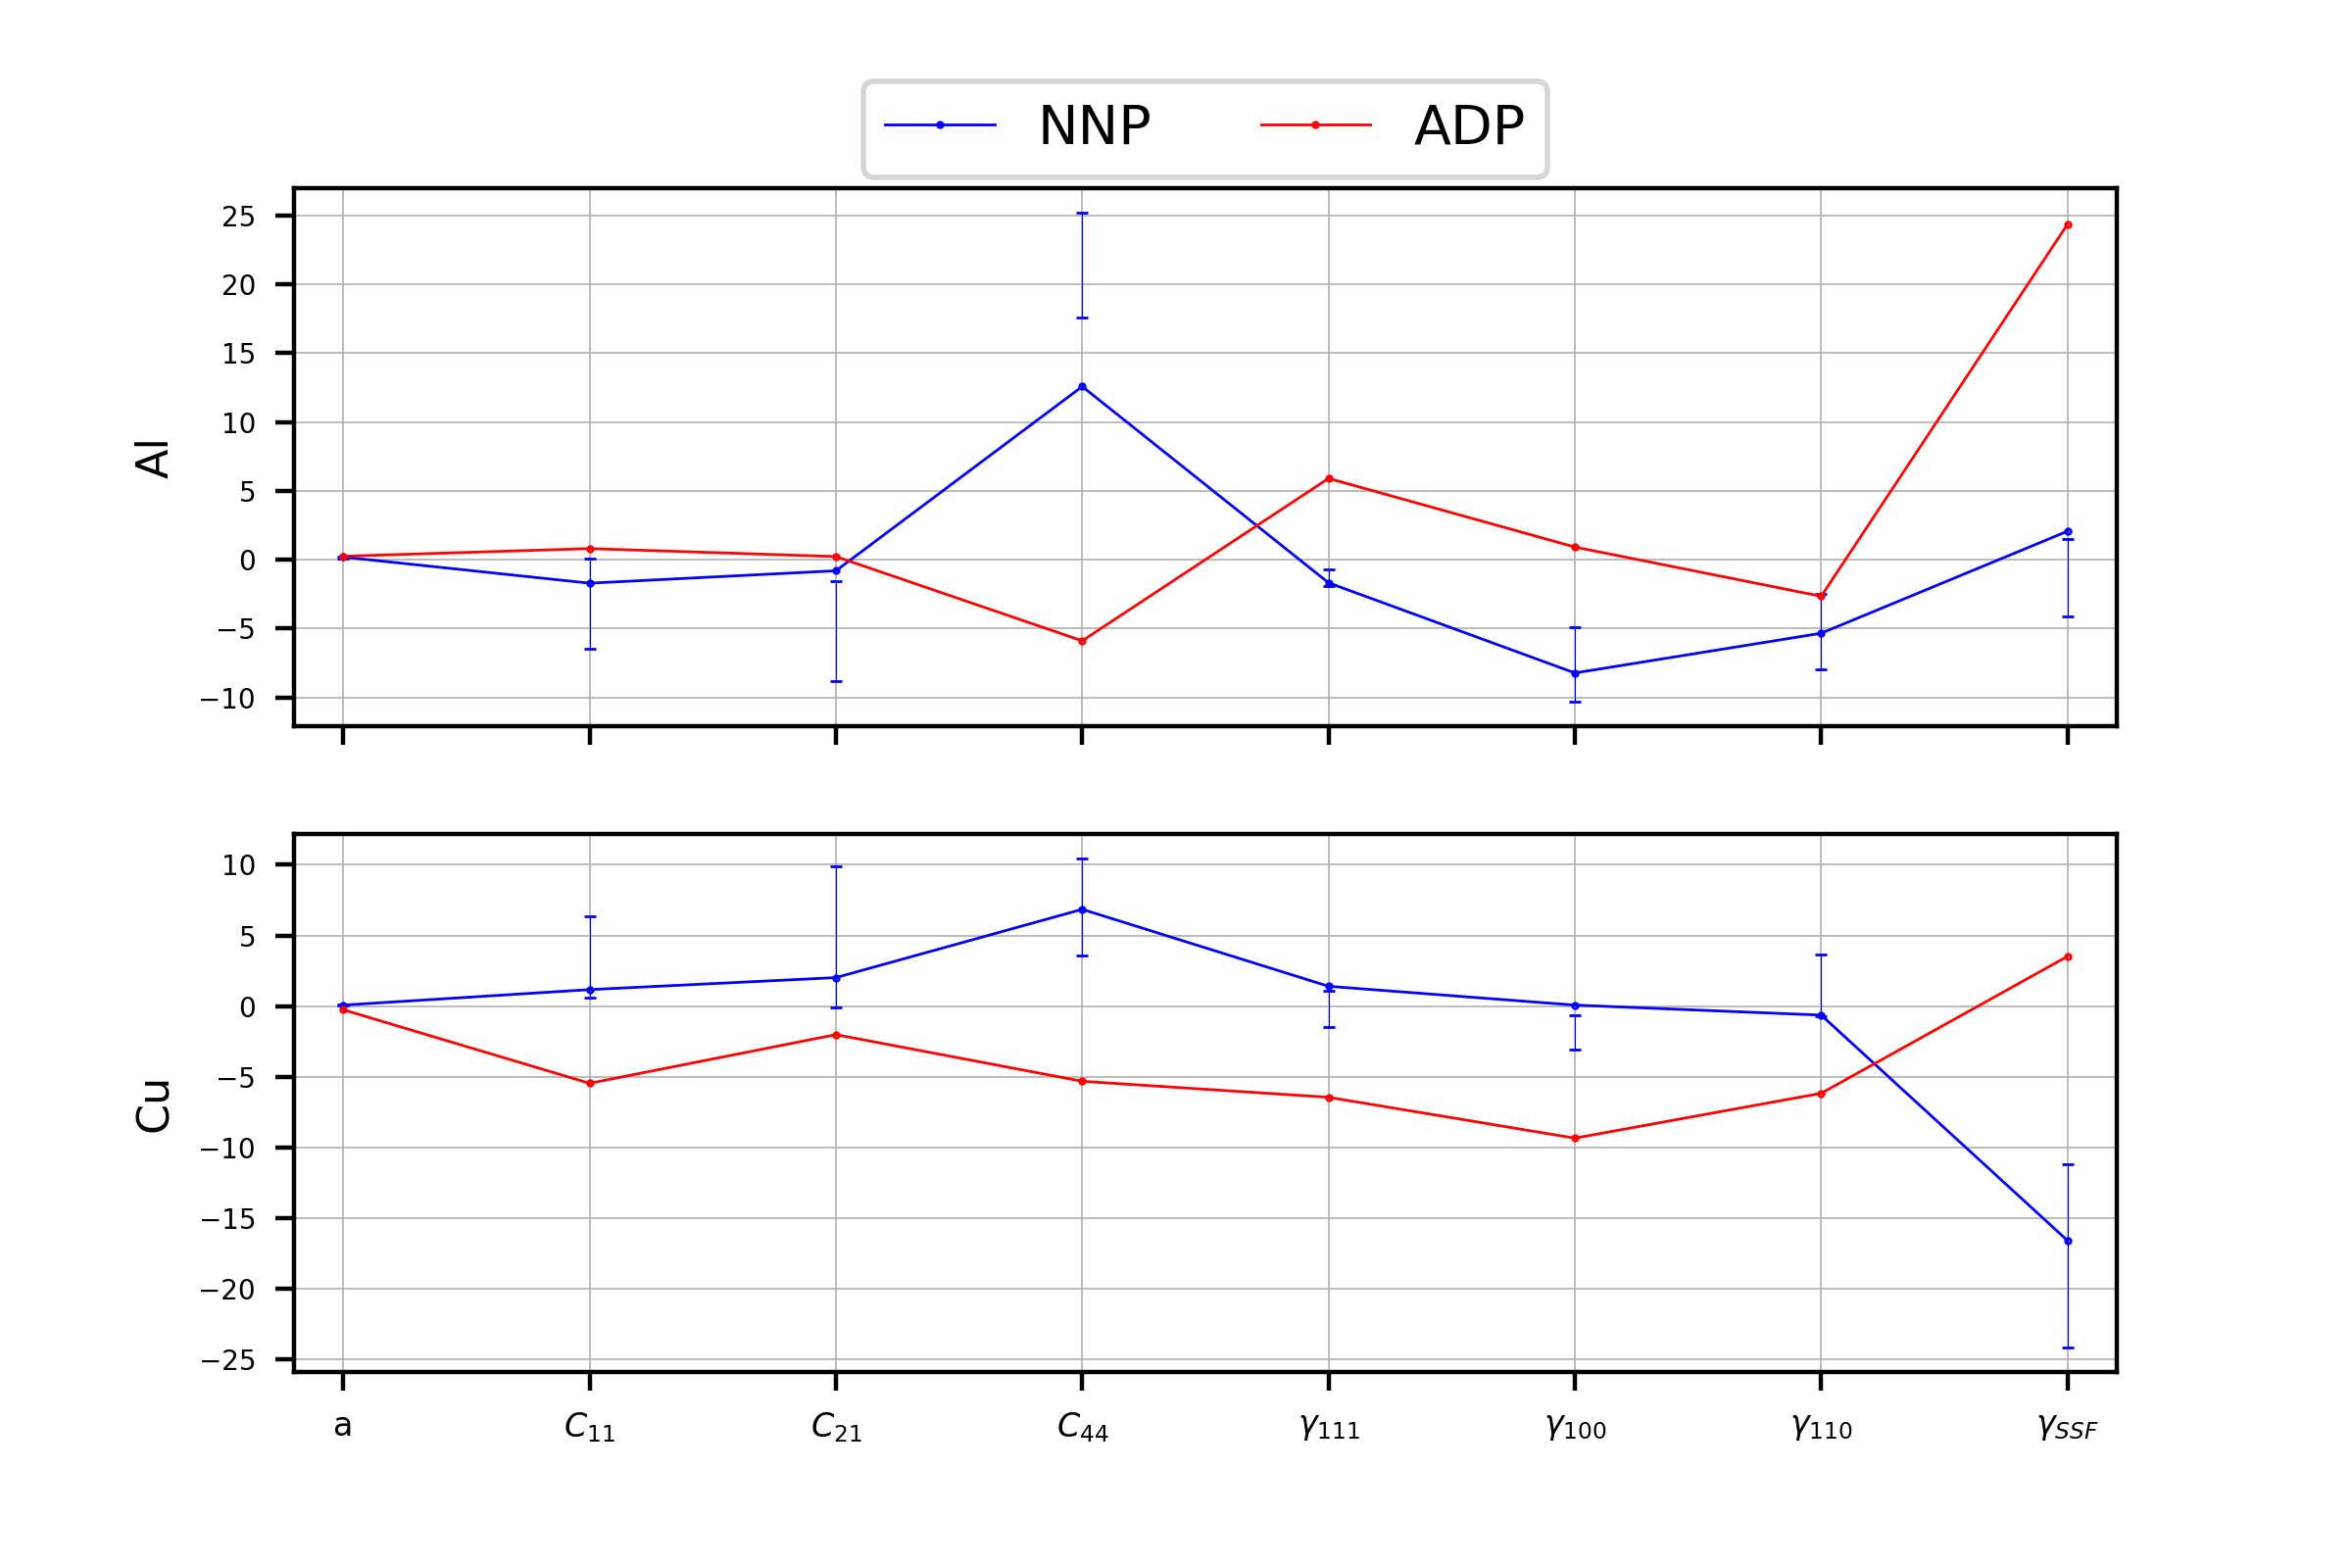
\includegraphics[width=1.2\textwidth,center]{./figures/matparam_purestats.png}%
\caption{Deviation of NNP and ADP from DFT (\%) for fundamental properties for Al and Cu. 
Relevant structures are included in the training set. }%
\label{fig:matparam_purestats}
\end{figure}
The NNP outperforms ADP for formation energy, atomic volume, and elastic constants for most OQMD structures, as can be seen in Figure \ref{fig:matparam_stats1}.
We compute structure formation energy $\Delta E^{structure}_f$ of all structures as relative to bulk FCC Al and dilute Cu in matrix:
\begin{equation} \label{eqn:formE_structure}
\Delta E^{structure}_f = E^{structure} - \sum_i E^{ref}_i
\end{equation}
\begin{equation} \label{eqn:formRef_Al}
E^{ref}_{Al} = E^{FCC}_{Al}
\end{equation}
\begin{equation} \label{eqn:formRef_Cu}
E^{ref}_{Cu} = E^{1sol}_{255Al,1Cu} - 255E^{FCC}_{Al}
\end{equation}
Formation energy is particularly well-handled by the NNP, with most errors well within a few meV/atom, while ADP often highly overestimates or underestimates the formation energy;
in a few cases, ADP reverses the sign, i.e., predicting stable compounds as unstable and vice versa.
However, for structures with high formation energy, both the NNP and ADP tend to struggle, often they do not end up relaxing to the same structure as DFT, or they have substantial errors.
ADP regularly underestimates the atomic volume, even for critical structures: $\theta$ and $\theta'$ errors can be substantial, see \textcolor{red}{supplementary table}.
For elastic constants, we see that neither ADP nor NNP performs ideally.
ADP does a reasonable job of capturing the precipitate structures and outperforms NNP on pure aluminum.
However, we see that ADP often makes quite substantial errors in the elastic constants for intermediate compounds, while this is less the case for NNP. Interestingly it seems that the B2 structure poses a challenge to both ADP and most NNP.
ADP predicts B2 to be extremely stable, while it has the highest error for any stable compound for NNP. 


\begin{figure}[H]%
\centering%
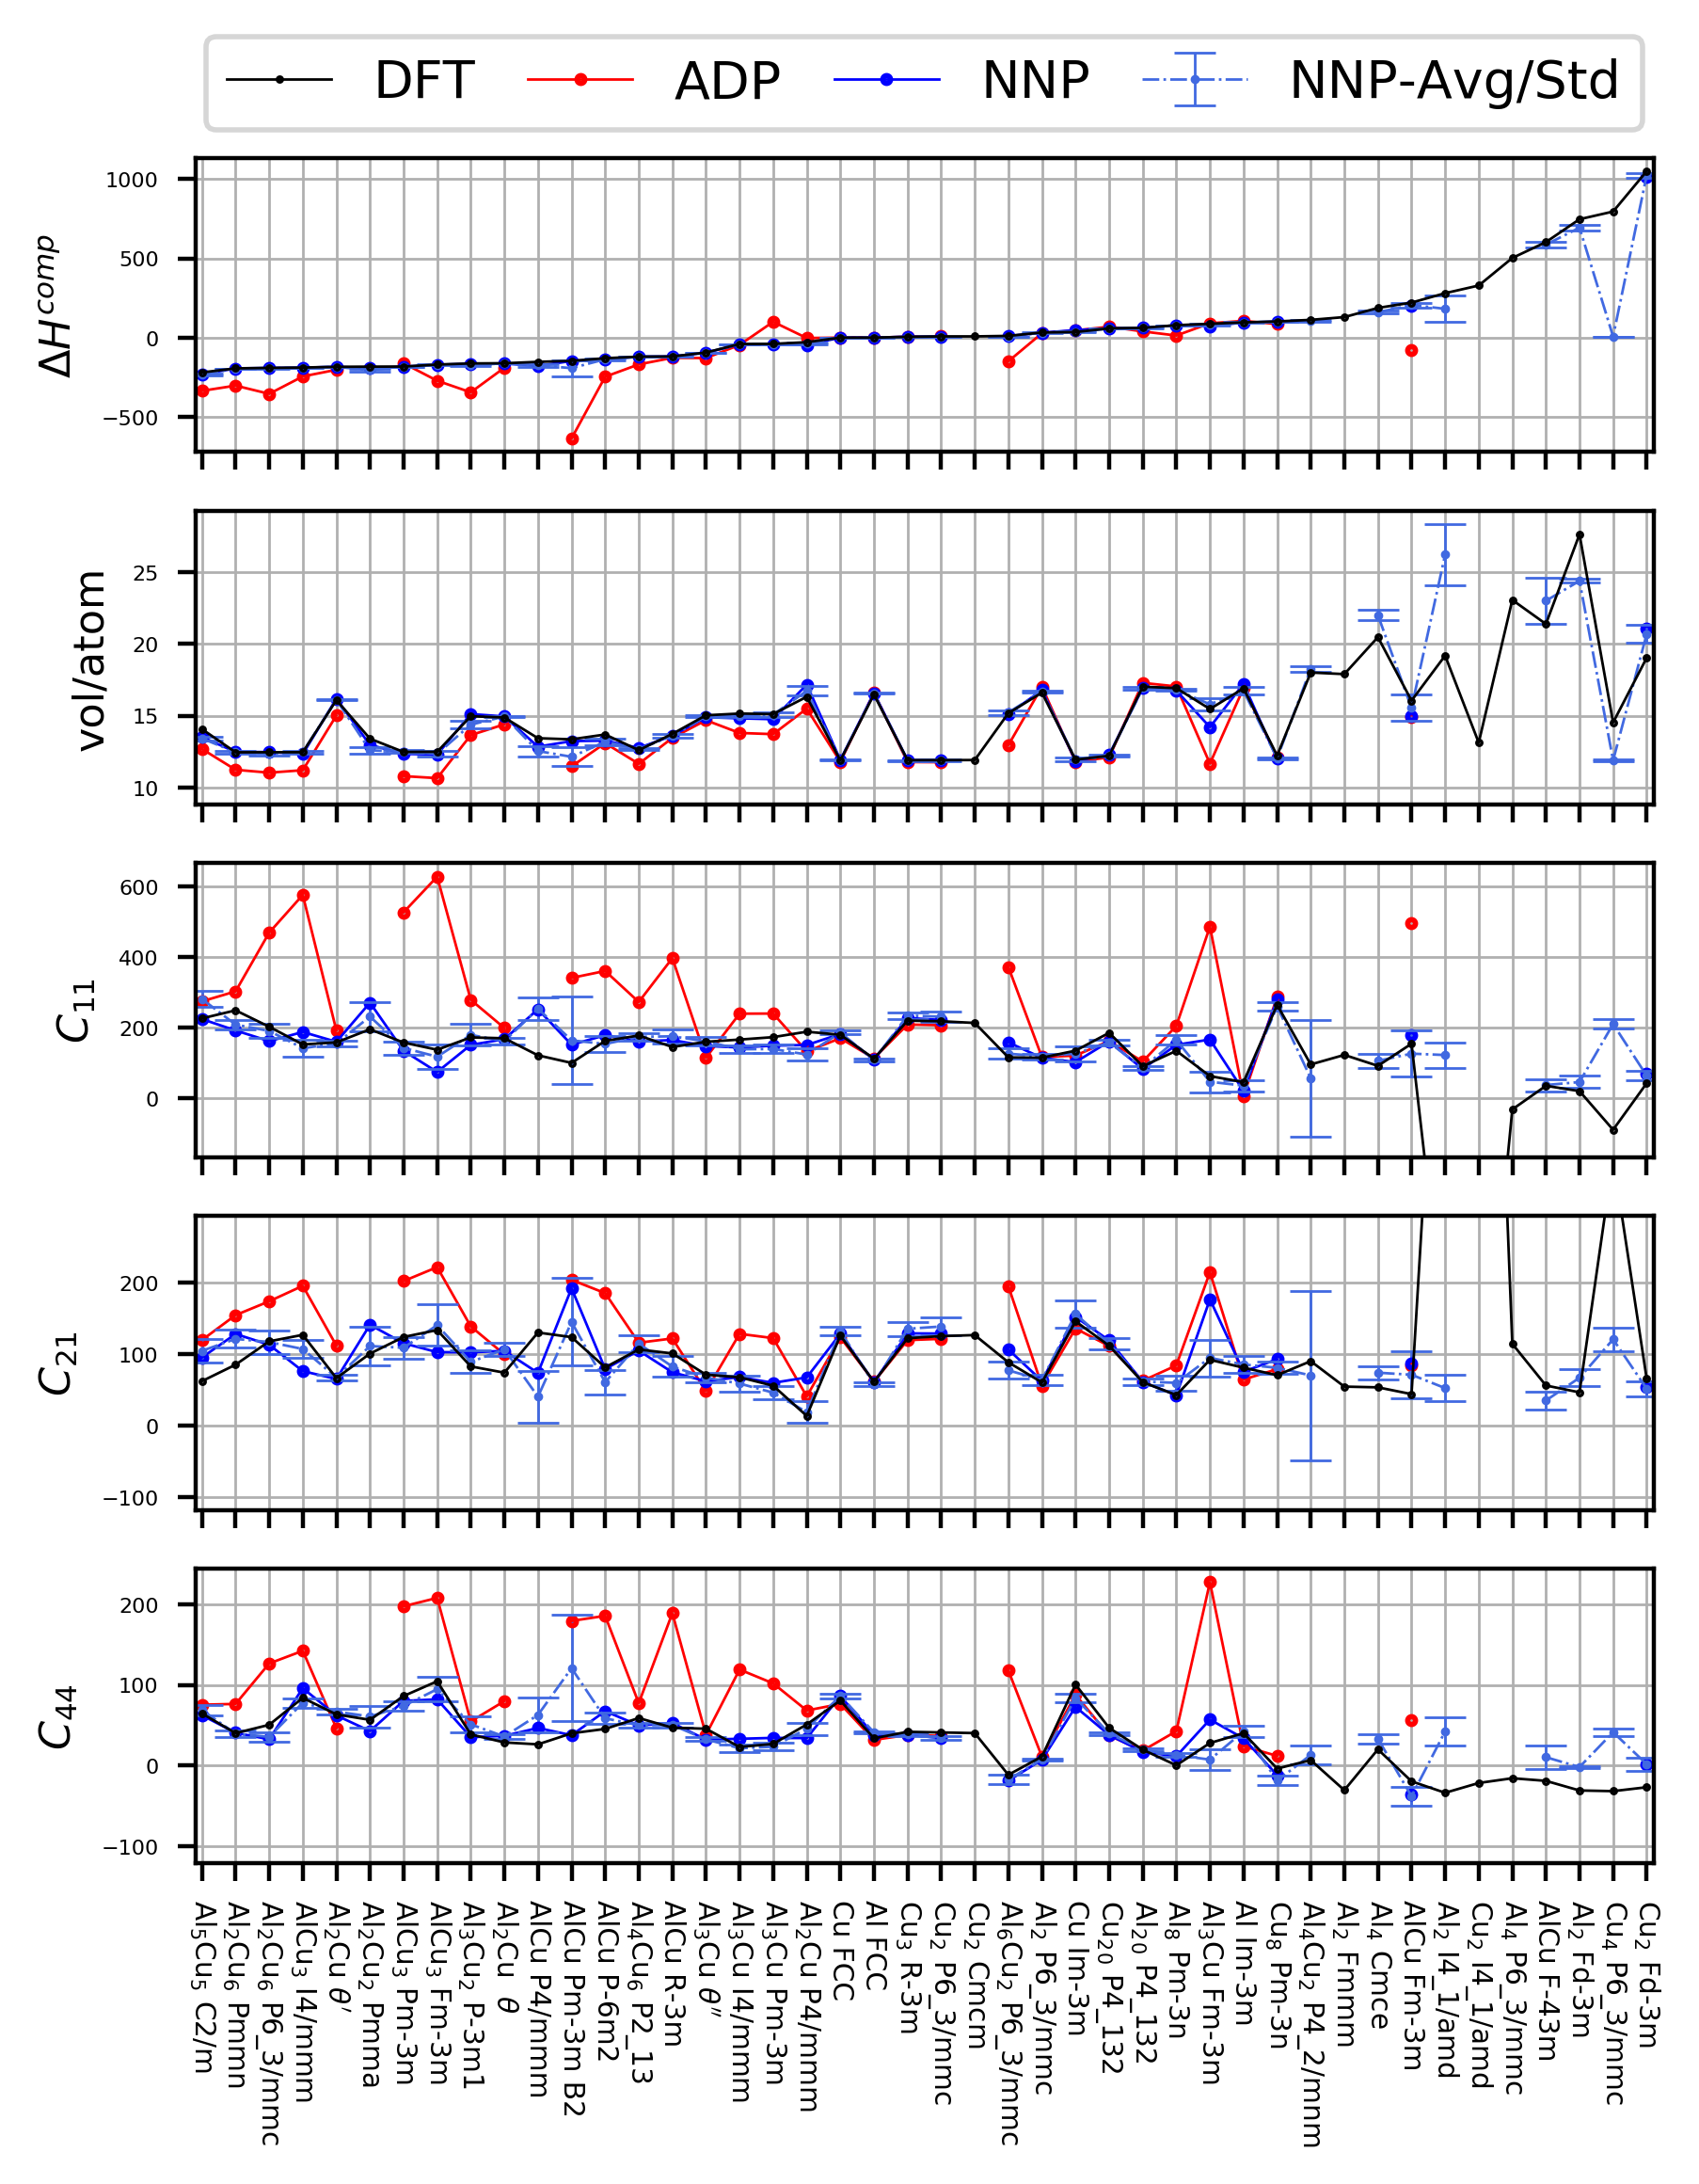
\includegraphics[width=1.2\textwidth,center]{figures/matparam_stats1.png}%
\caption{Comparison of: formation energy (meV), atomic volume (Ang$^3$), elastic constants C$_{11}$, C$_{21}$ and C$_{44}$ (GPa) across NNP, ADP and DFT for all structures in the OQMD. 
Relevant structures are included in the training set. }
\label{fig:matparam_stats1}
\end{figure}

The binary formation energies for Cu, Al, and Vacancy in Al or Cu matrix was computed with following:
\begin{equation}
\Delta E^{bind}_f = E^{2sol}_{N-2,X,Y}-E^{1sol}_{N-1,X}-E^{1sol}_{N-1,Y}+E^{pure}_N
\end{equation}
Note for Al-matrix results this is the same as equation \ref{eqn:formE_structure}, while for 
Cu-matrix results the reference is swapped to Cu matrix and Al solute.
Also, due to Cu having a much higher computational cost, reference is to a 108 atom 3x3x3 supercell.
The results for Al matrix are displayed in Figure \ref{fig:solsol_in_al} while those for Cu matrix are contained in the \textcolor{red}{Figure S \ref{fig:solsol_in_cu}}.
For the solute binding, we see that the NNP, while not always ideal, more closely matches DFT.
Particularly for dilute Cu-Cu binding, ADP falsely predicts massive overbinding for near neighbors and massive repulsion for further neighbors, while NNP maintains quantitative accuracy.
Errors for NNP are typically in the 20-30 meV range, and values requiring greater precision than this would not be appropriate for NNP.


\begin{figure}[H]%
\centering%
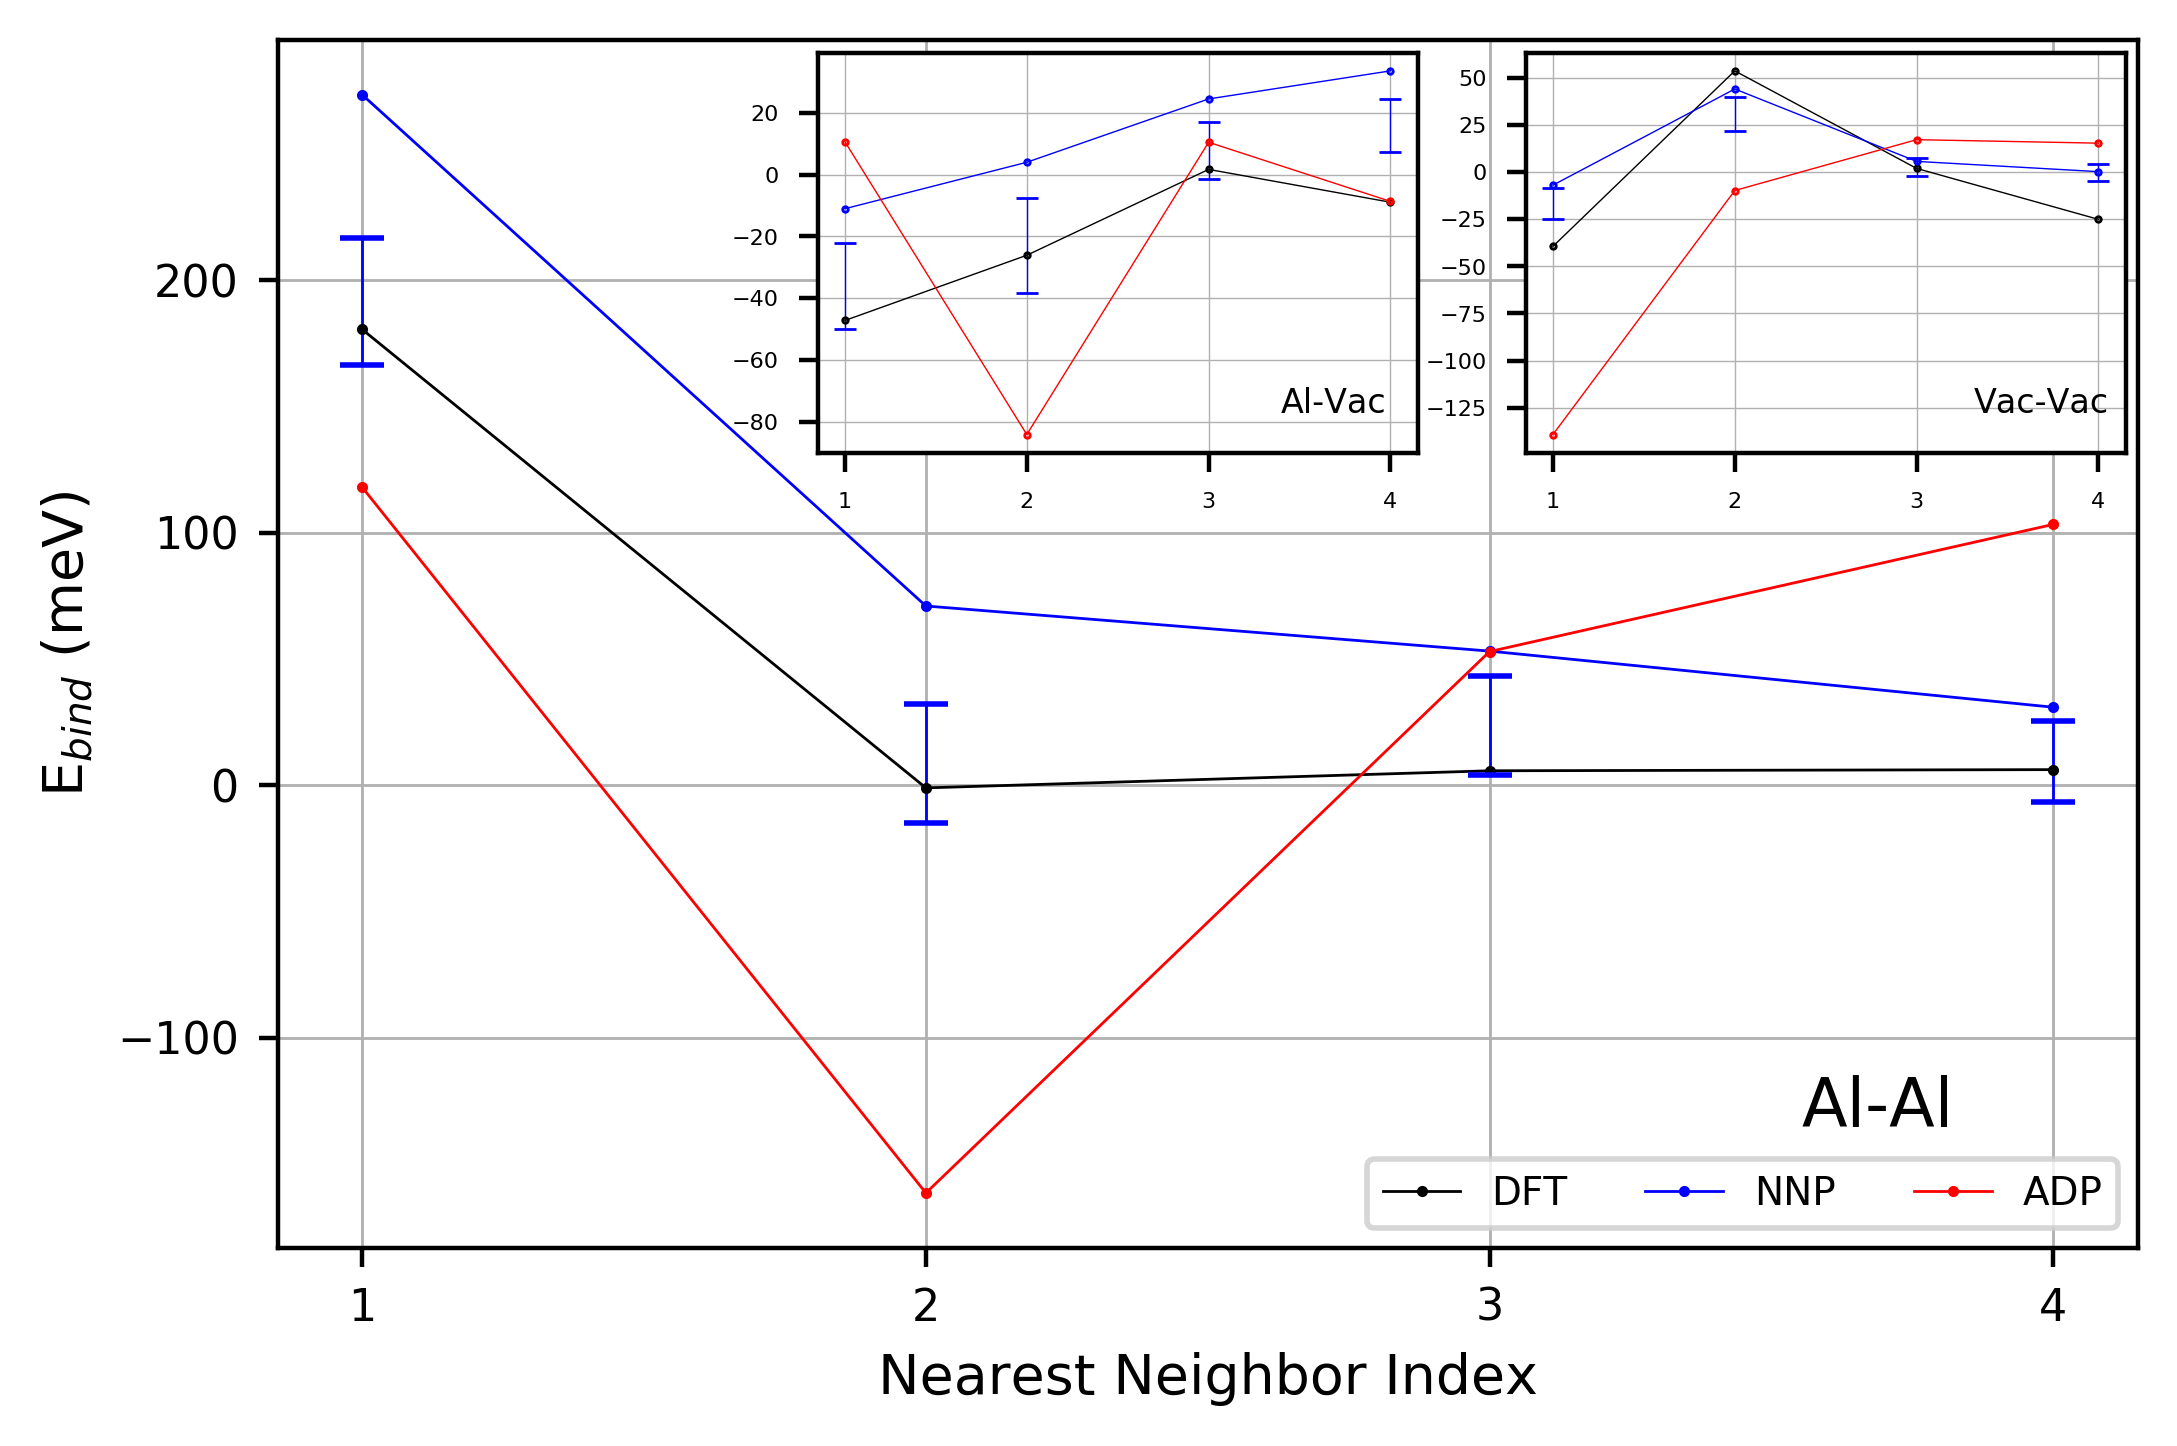
\includegraphics[width=1.2\textwidth,center]{./figures/solsol_in_al.png}%
\caption{Neighbor index vs. binding energy $E_{bind}$ for Cu-Cu, Cu-Vac and Vac-Vac in Al matrix. 
Relevant structures are included in the training set.}%
\label{fig:solsol_in_al}
\end{figure}

\textcolor{red}{Not yet sure whether geometry has a separate section or not}.
In this work, the coherent and semi-coherent versions of the $\theta''$ and $\theta'$ interfaces were studied while $\theta$ was omitted since it only forms incoherent interfaces \cite{Nie2014PhysicalAlloys}.
We constructed these interfaces by taking their OQMD entries and stacking them on the Al matrix using the ASE \mintinline{python}{ase.build.stack} command.
During relaxation, atoms are free to move, but the cell is held fixed. 
Reference images for these interfaces are included in \textcolor{red}{Figure XX} in the supplementary.

We computed the interface energy in the same manner as in \cite{Vaithyanathan2004MultiscaleAlloys}, and we only briefly summarize the method here.
The formation energy for an interface with N atoms of which X are of the matrix and Y are of the precipitate,
$\Delta E^{interface}_{f, (X,Y)} = E^{interface}_{X,Y}-XE^{Matrix}_{bulk}-YE^{Precip}_{bulk}$,
is related to the number of atoms in the following equation. 
\begin{equation}
\Delta E^{interface}_{f,(X,Y)} = \delta E^{strain}_{X,Y} + \frac{2A\gamma^{interface}}{N}
\end{equation}
Where $\Delta E^{interface}_f$ is the interface formation energy, $\delta E_{strain}$ is the strain energy, $A$ the surface area,
$\gamma^{int}$ the interface energy, and $N=X+Y$ the total number of atoms in interface.
The interface surface energy $\gamma^{interface}$ is then the slope of $\frac{1}{N}$ against
$\Delta E^{interface}_f$, divided by $2A$.
We calculated the slope using three different sizes of the $\theta'$ structures and four different sizes of $\theta''$ structures, starting with a minimum of one precipitate layer and two Al layers and incrementing onward in size. 


%\setlength{\tabcolsep}{20pt}
%\setlength{\tab}{20pt}
\textcolor{red}{TODO: Misfit vol definition}
\textcolor{red}{TODO: Cluster Energy definition}
\textcolor{red}{TODO: Sol-SF Energy defintion}
\begin{equation}
\Delta E^{cluster}_{f,(N-X,X)} = E^{cluster}_{N-X,X} - \sum_i E^{ref}_i
\end{equation}
\begin{equation}
\Delta E^{Sol-SF}_{f,(N-1,X)} = E^{Sol-SF}_{N-1,1} - E^{SF}_{N} - (E^{Pristine}_{N-1,1}-E^{Pristine}_{N})
\end{equation}



\begin{table}[h!]
\begin{tabular}{l|cccc}%
\hline%
&DFT&ADP&NNP& NNP-\emph{Avg / StdDev}\\%
\hline%
Misfit Vol Cu in Al ($\AA^3$)&{-}5.770&{-}16.958&{-}4.380&\emph{-7.095 / 1.076}\\%
Misfit Vol Al in Cu ($\AA^3$)&2.421&{-}1.259&0.109&\emph{1.334 / 0.857}\\%
$E^{3Cu}_{111}$ (eV)&{-}0.073, \emph{-0.09}\cite{Gorbatov2019EffectiveAlloys}&{-}0.718&{-}0.112&\emph{-0.060 / 0.037}\\%
$E^{3Cu}_{112}$ (eV)&{-}0.112, \emph{-0.13}\cite{Gorbatov2019EffectiveAlloys}&{-}0.595&{-}0.097&\emph{-0.085 / 0.025}\\%
$E^{4Cu}_{111111}$ (eV)&\emph{0.06}\cite{Gorbatov2019EffectiveAlloys}&{-}0.612&{-}0.081&\emph{0.071 / 0.086}\\%
$E^{4Cu}_{111112}$ (eV)&\emph{-0.17}\cite{Gorbatov2019EffectiveAlloys}&{-}1.071&{-}0.184&\emph{-0.093 / 0.066}\\%
$E^{4Cu}_{111122}$ (eV)&\emph{-0.34}\cite{Gorbatov2019EffectiveAlloys}&{-}1.275&{-}0.226&\emph{-0.205 / 0.055}\\%
SolSF Cu in Al (eV)&0.052&0.108&0.042&\emph{0.062 / 0.030}\\%
SolSF Al in Cu (eV)&{-}0.049&{-}0.034&{-}0.006&\emph{0.002 / 0.031}\\%
\label{table:solute_special}
\end{tabular}%
\caption{Misfit Volumes, Cu cluster energies and solute-stacking fault interactions for DFT, ADP and NNP}
\end{table}


Figure \ref{fig:interface_energies} plots the results of the interface energy calculations.
ADP correctly predicts the general trends but makes several serious errors.
The coherent $\theta'$ interface has much too high an energy, while all the $\theta''$ interface is predicted to have negative energy.
The $\theta''$ interface is particularly challenging because it has such low interface energy; therefore, it is easy for the potential to predict this to be negative rather than positive.
However, our representative NNP has high quantitative accuracy on all these interfaces.

\begin{figure}[H]%
\centering%
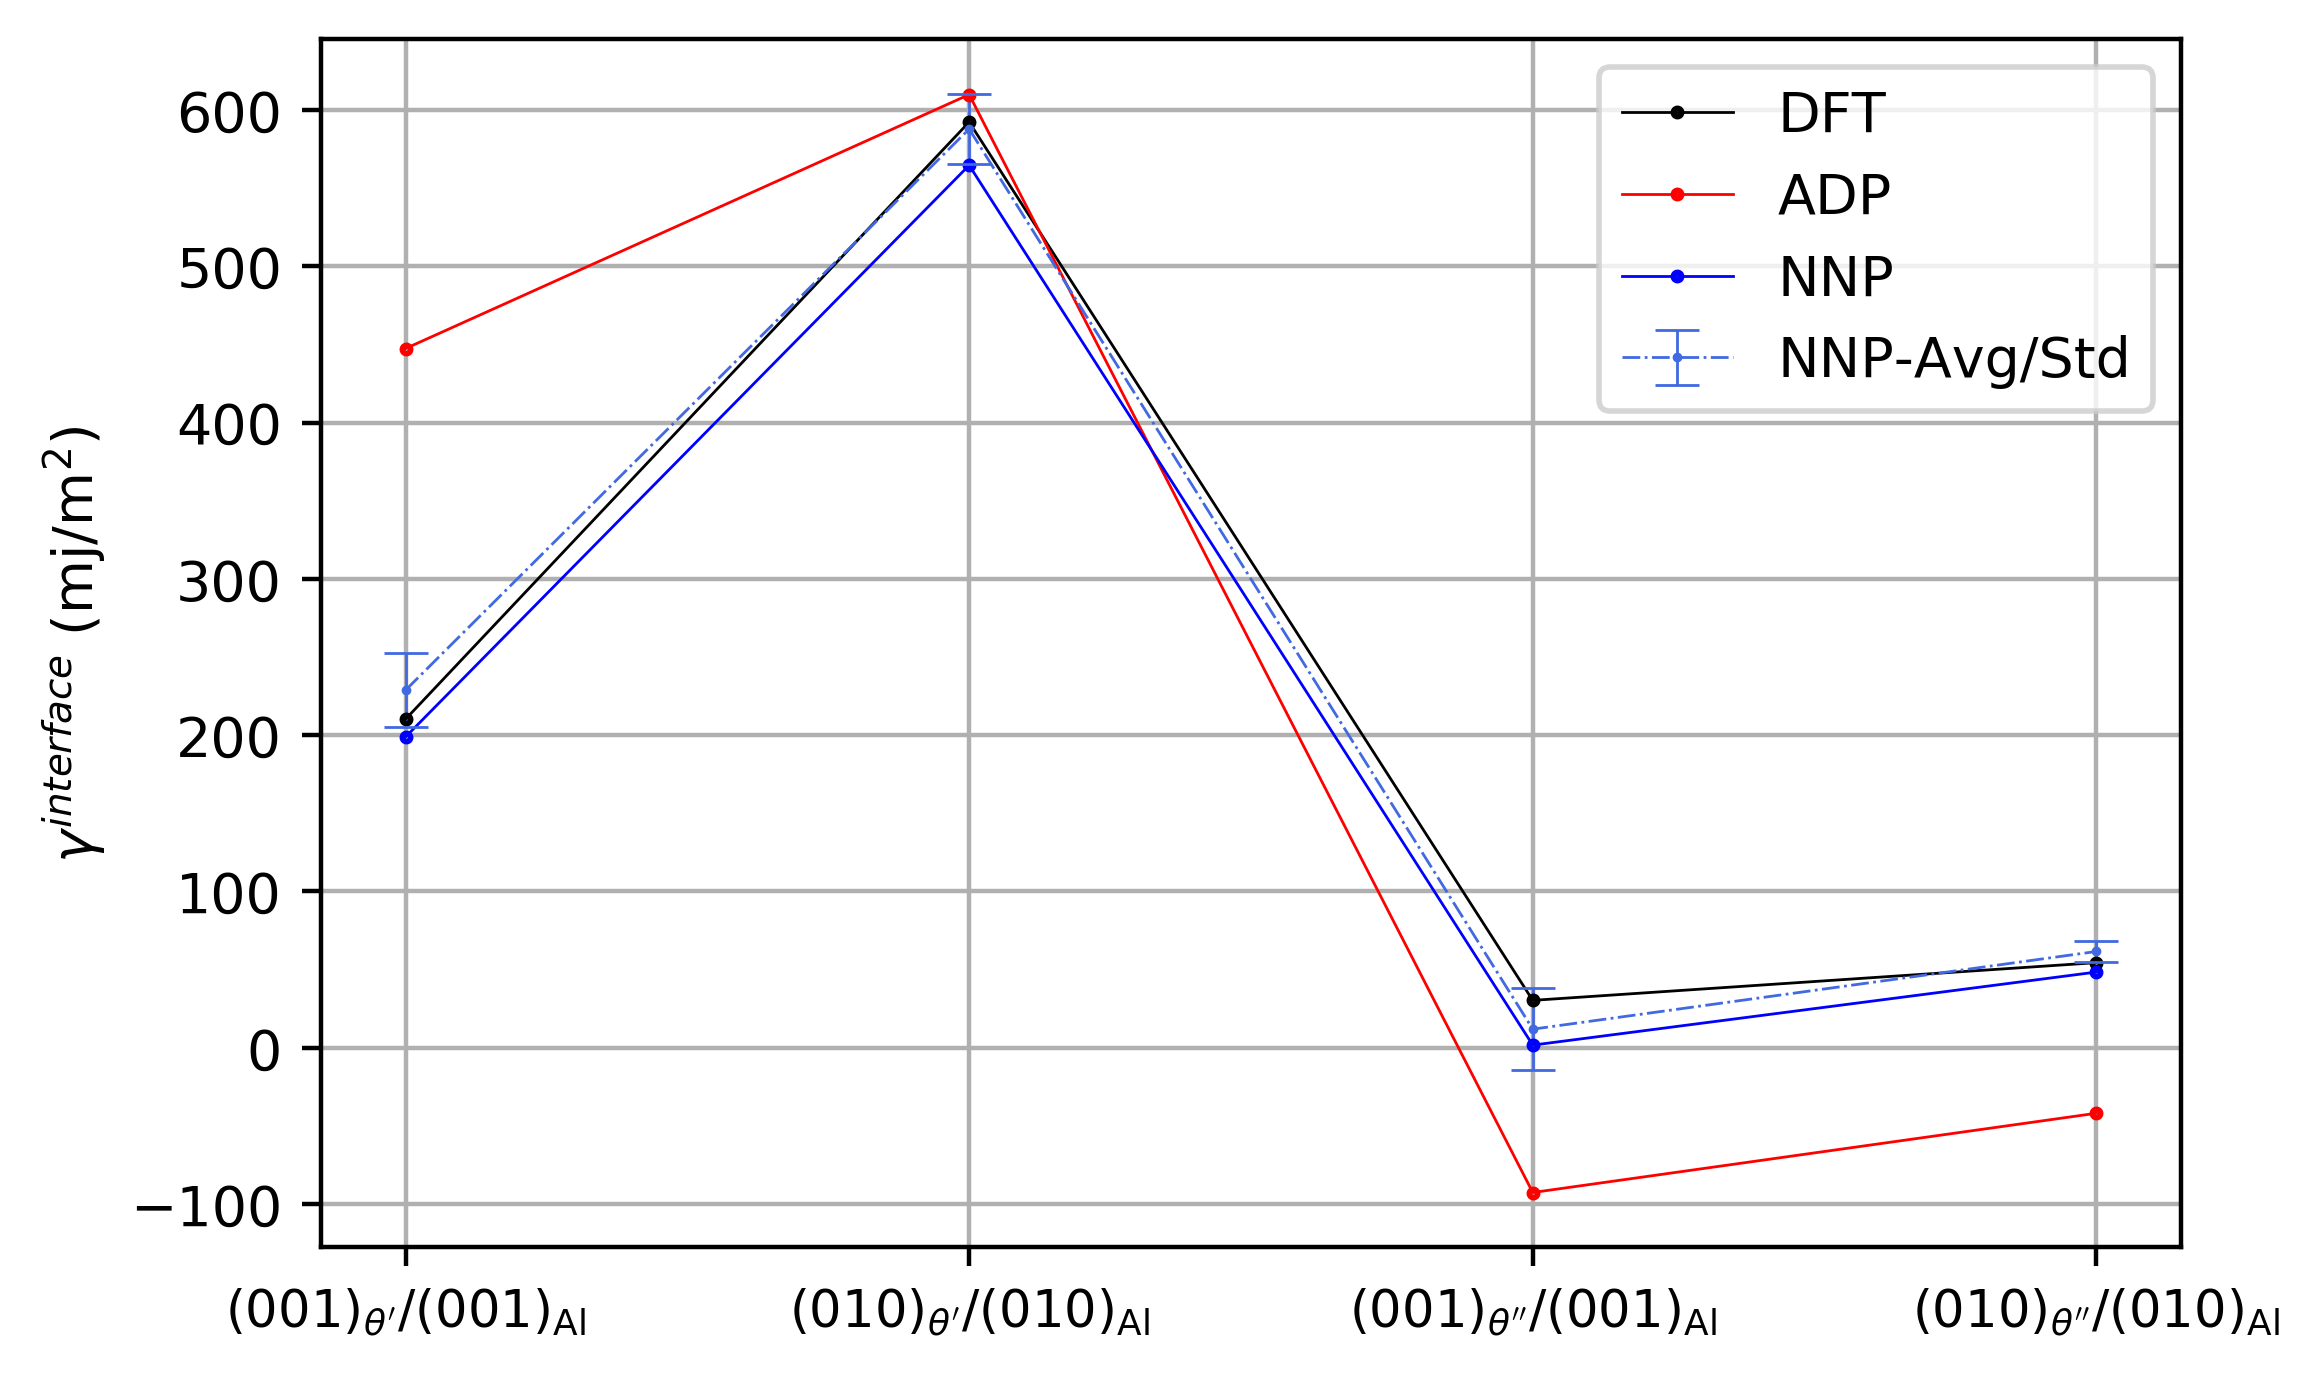
\includegraphics[width=1.2\textwidth,center]{./figures/interface_energies.png}%
\caption{Interface structure vs. interface energy for precipitate structures. 
These are the $\theta'$ coherent, $\theta'$ semi-coherent, $\theta''$ coherent and $\theta''$ semi-coherent
interfaces in order. Relevant structures are included in the t/raining set.}%
\label{fig:interface_energies}
\end{figure}

The $\theta''$ structure is the same as that of FCC aluminum, except that every second (100) plane is replaced with Copper.
The most mechanically-relevant GSF surface is that which coincides with the (111) plane of aluminum, which we display in Figure \ref{fig:GSF_ThetaDP_111} (b).
To compute the GSF energy surface, we follow the procedure detailed in \cite{Yin2017a}, which we briefly summarize here.
Firstly, the base cell was set up such that the z-direction was normal to the surface of interest while maintaining full periodicity.
Then for each point $\vec{R}$ on the GSF surface \textcolor{red}{a3 ADD DEFINITION} vector was correspondingly shifted, then both the atoms and the a3 cell vector were allowed to relax, but only in the z-direction.
The GSF energy at a displacement $\gamma_{GSF\vec{R}}$ was calculated using: 
\begin{equation}
\gamma^{GSF}_{\vec{R}} = (E^{GSF}_{\vec{R}} - E^{pristine})/A
\end{equation}
Where $E^{GSF}_{\vec{R}}$ is the total energy of the GSF displaced at $\vec{R}$, $E_{pristine}$ is the 
energy of the pristine structure without deformation, and $A$ is the area spanned by the GSF surface.
In \ref{fig:GSF_ThetaDP_111} (a), we see the results for the entire GSF surface.
The NNP potential gives a smooth GSF, with clear peaks and valleys in the energy corresponding with the underlying atomic positions.
The ADP potential, conversely, is substantially less smooth; there is also a noticeable lack of radial symmetry and high and low energy sites,  with cobweb-like extensions across high energy points.
Most troubling for ADP, is that regions of the $\theta''$ surface are unphysically negative in energy, this severely compromises ADP to give high-quality results for dislocation-precipitate interactions.
Importantly, NNP gives highly accurate energies, even though we did not train the NNP for this GSF surface.
A further example of using the NNP for GSF prediction is in \textcolor{red}{supplementary X}

\begin{figure}[H]%
\centering%
\subfloat[]{{
 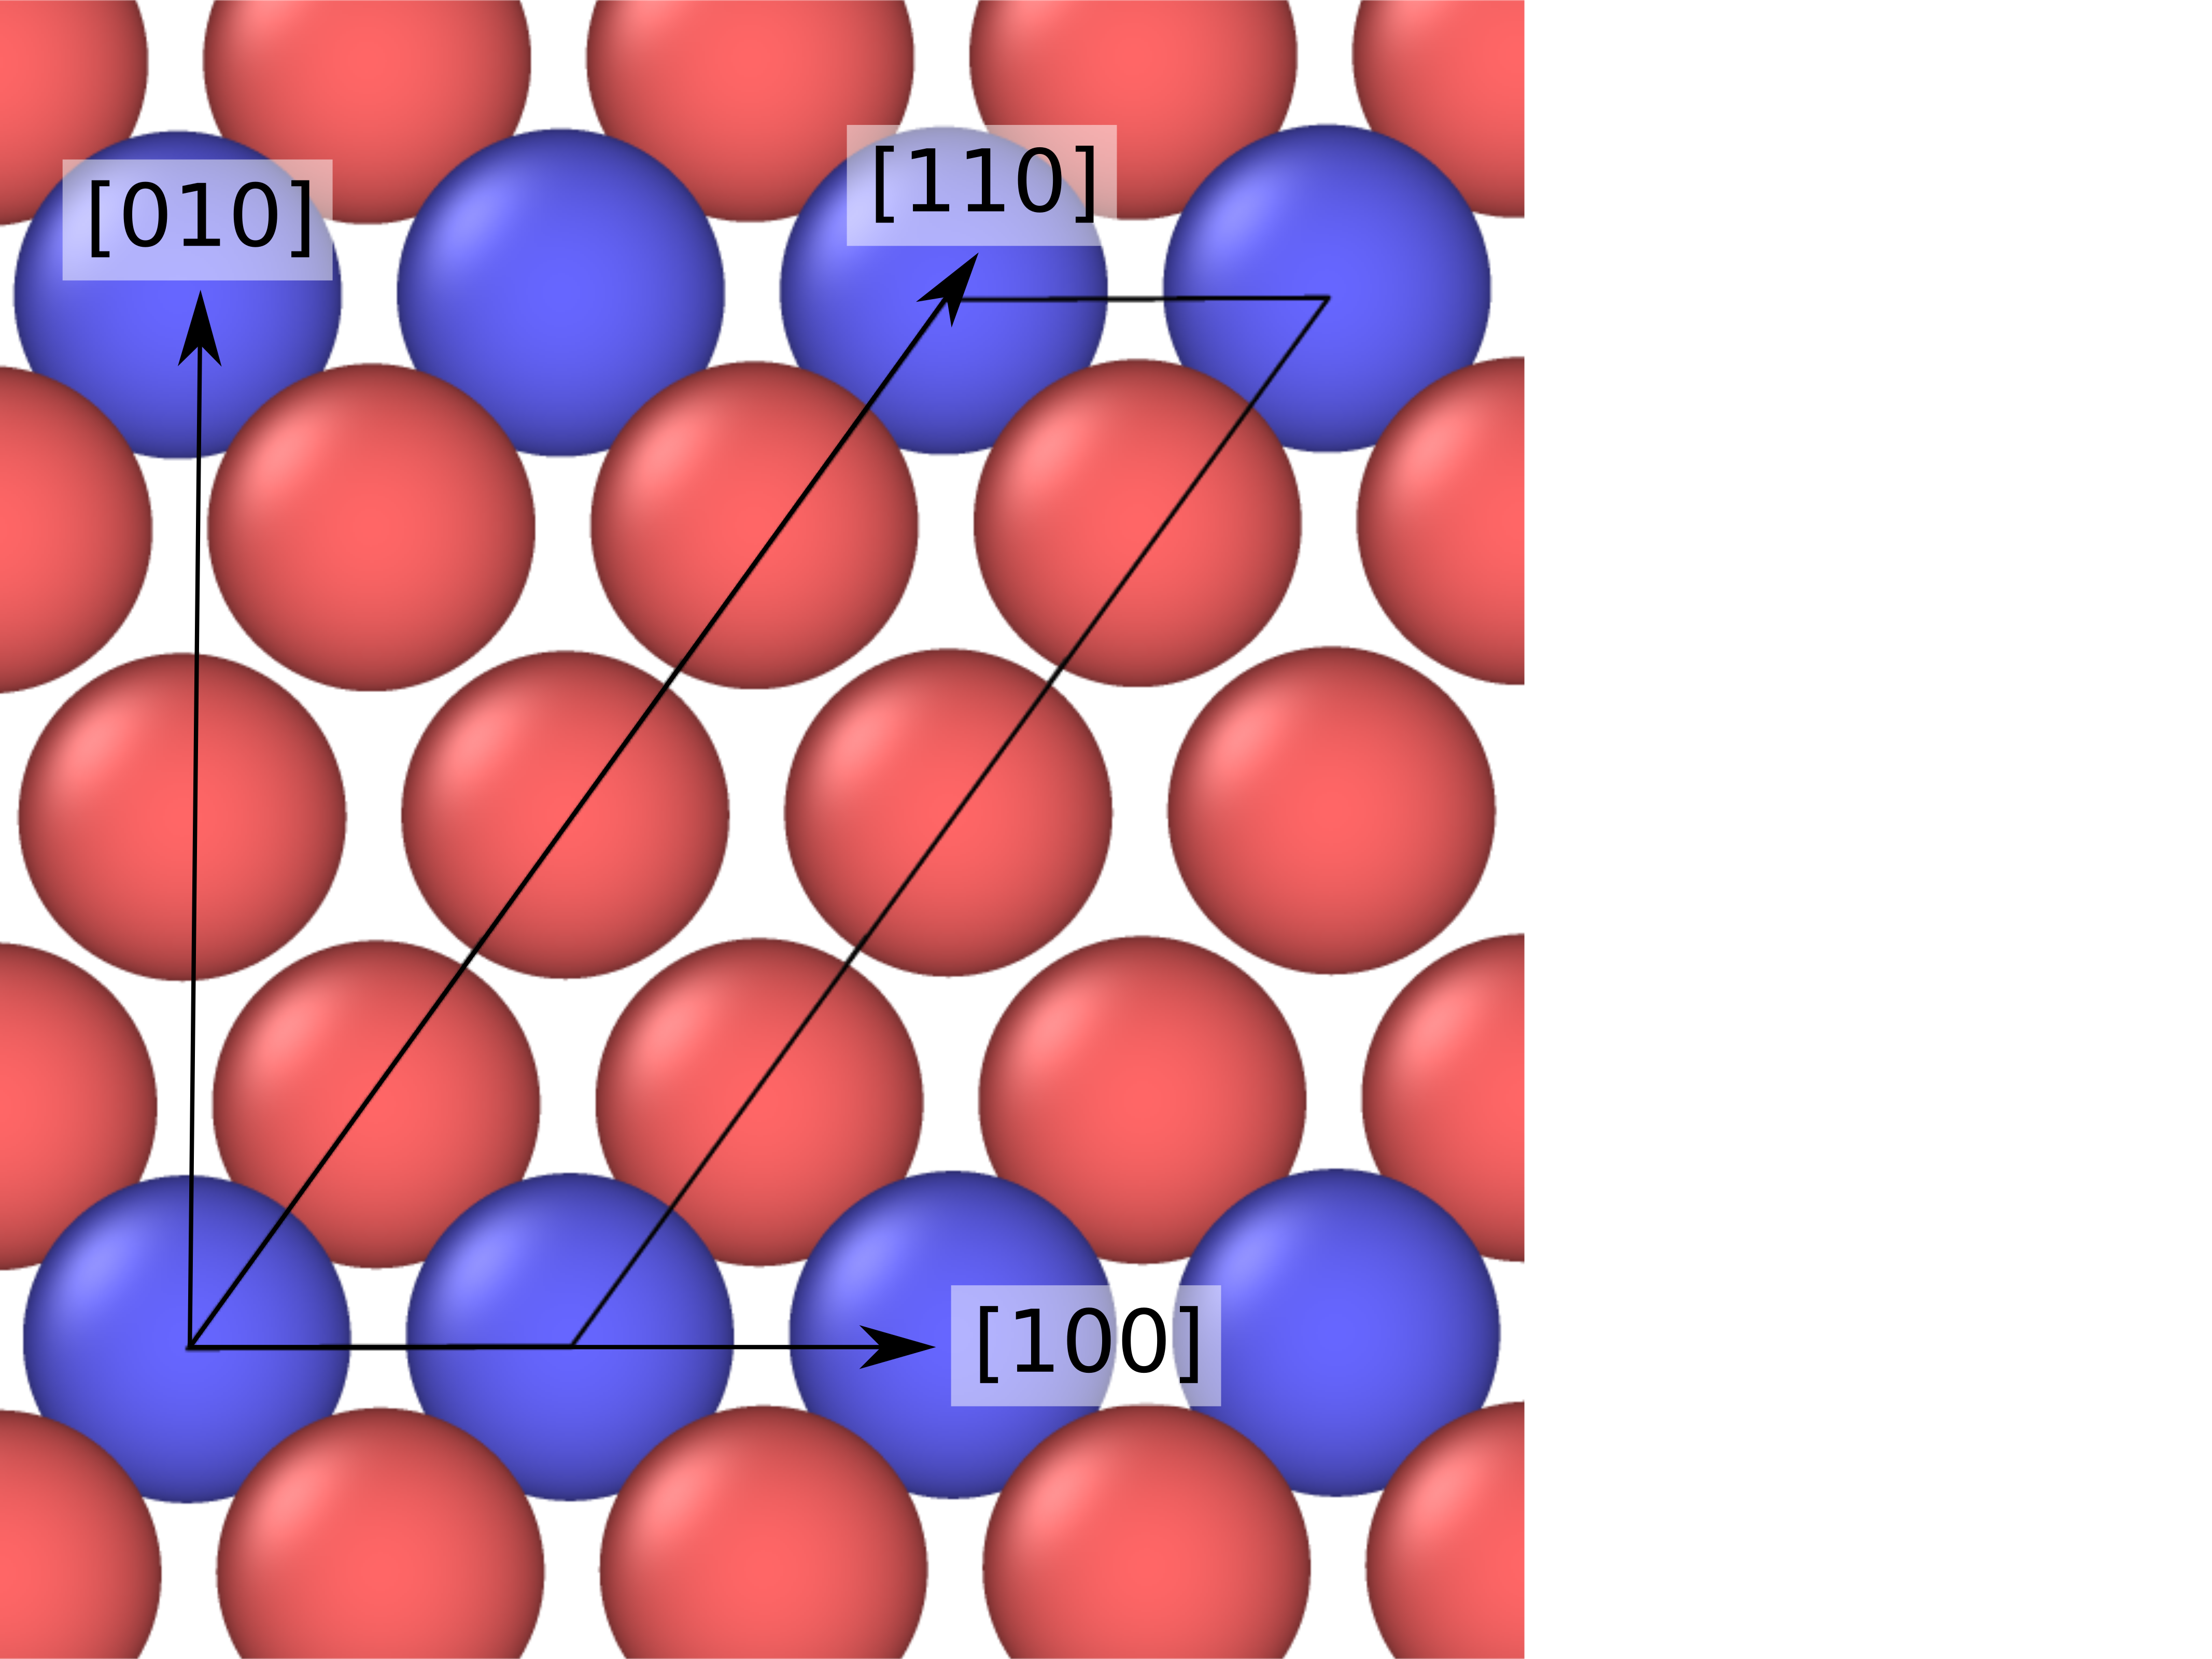
\includegraphics[width=0.25\textwidth]{figures/GSF_ThetaDP111_AtomicView.png}
 }}%
\subfloat[]{{
 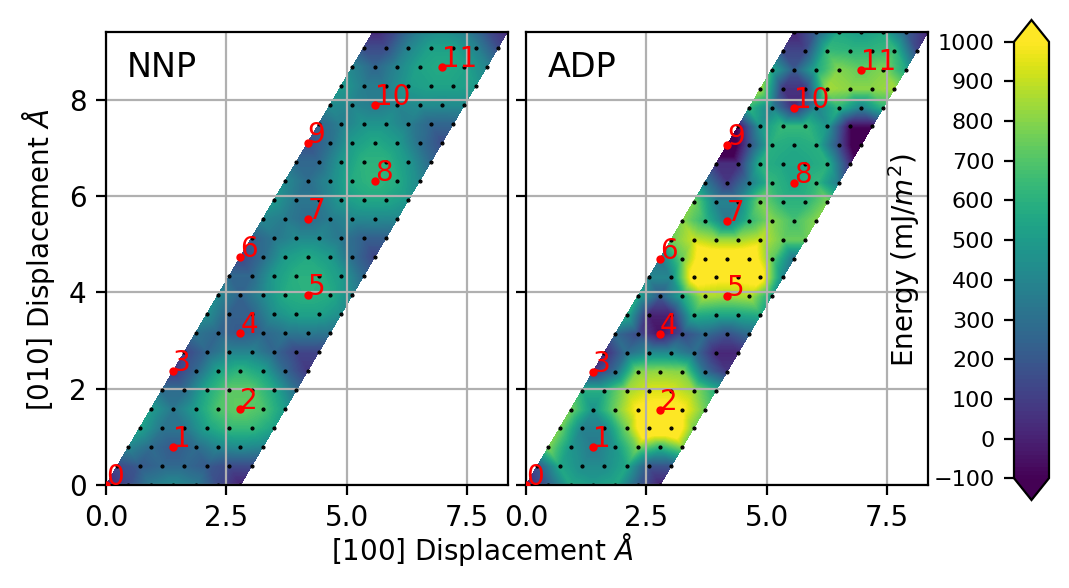
\includegraphics[width=0.75\textwidth]{figures/GSF_ThetaDP111_surf.png}
 }}%
\\
\subfloat[]{{
 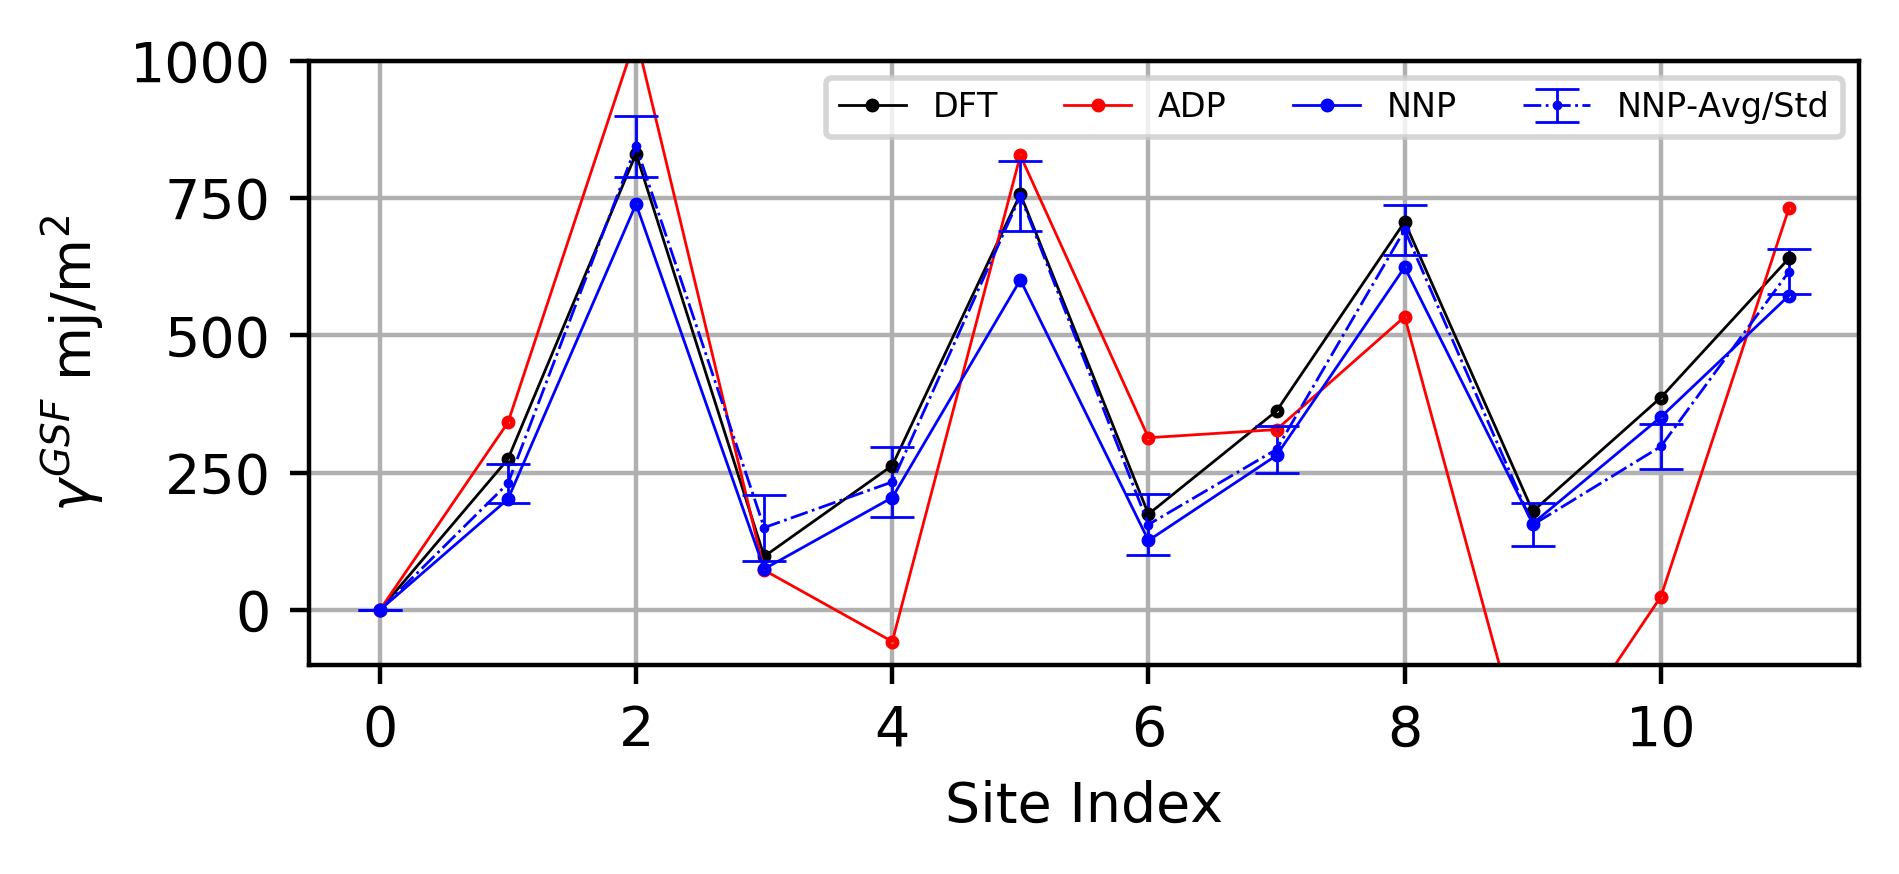
\includegraphics[width=1.00\textwidth]{figures/NOTINOQMD_00002-GSF_111.png}
 }}%
\caption{(a) GSF energy and (b) atomic coordinates for the $\theta''$ (111) surface. 
In (b), each black dot represents a point of calculation for NNP and ADP, while the red numbered dots are sites that were computed with DFT.
(c) Site index vs. GSF energy for DFT, NNP, and ADP.
While bulk $\theta''$ was included
in training set, the GSF calculations were not.}
\label{fig:GSF_ThetaDP_111}
\end{figure}

Antisites were computed for every OQMD structure in the following manner.
Firstly, the structure was allowed to be completely relaxed.
If the structure maintained the same symmetry group after full cell and atomic relaxation, we analyzed it for unique atomic sites using pymatgen.
Then the cell was duplicated, such as to generate cells with a minimum of 108 atoms to minimize defect-defect interactions.
For each of the unique sites identified, we then swapped it with the different atom, e.g., Al $\rightarrow$ Cu or Cu $\rightarrow$ Al, else we deleted the site to generate a vacancy and stored the antisite structure.
The energies of all antisite structures were calculated without relaxation.
This equation gave the antisite formation energies $\Delta E^{antisite}_f$:
\begin{equation}
\Delta E^{antisite}_f = E_{antisite} - E_{pristine} - \sum\Delta n_i E^{ref}_i
\end{equation}
Where $E^{antisite}$, $E^{pristine}$ are the total energies of the antisite, and pristine structure, $n_i$ is the 
number and sign of the swapped atoms, and $E^{ref}_i$ is the reference energy for compound $i$, as stated in 
equations \ref{eqn:formRef_Al} and \ref{eqn:formRef_Cu}.

Figure \ref{fig:antisite_plot} shows the antisite results.
\textcolor{red}{NNP attains excellent accuracy despite the lack of training data.
Error bars rarely exceed 5meV and are almost always centered around the correct DFT value.
ADP also performs reasonably but has substantially more errors, with many samples deviating more than 10meV/atom from DFT. }

\begin{figure}[H]%
\centering%
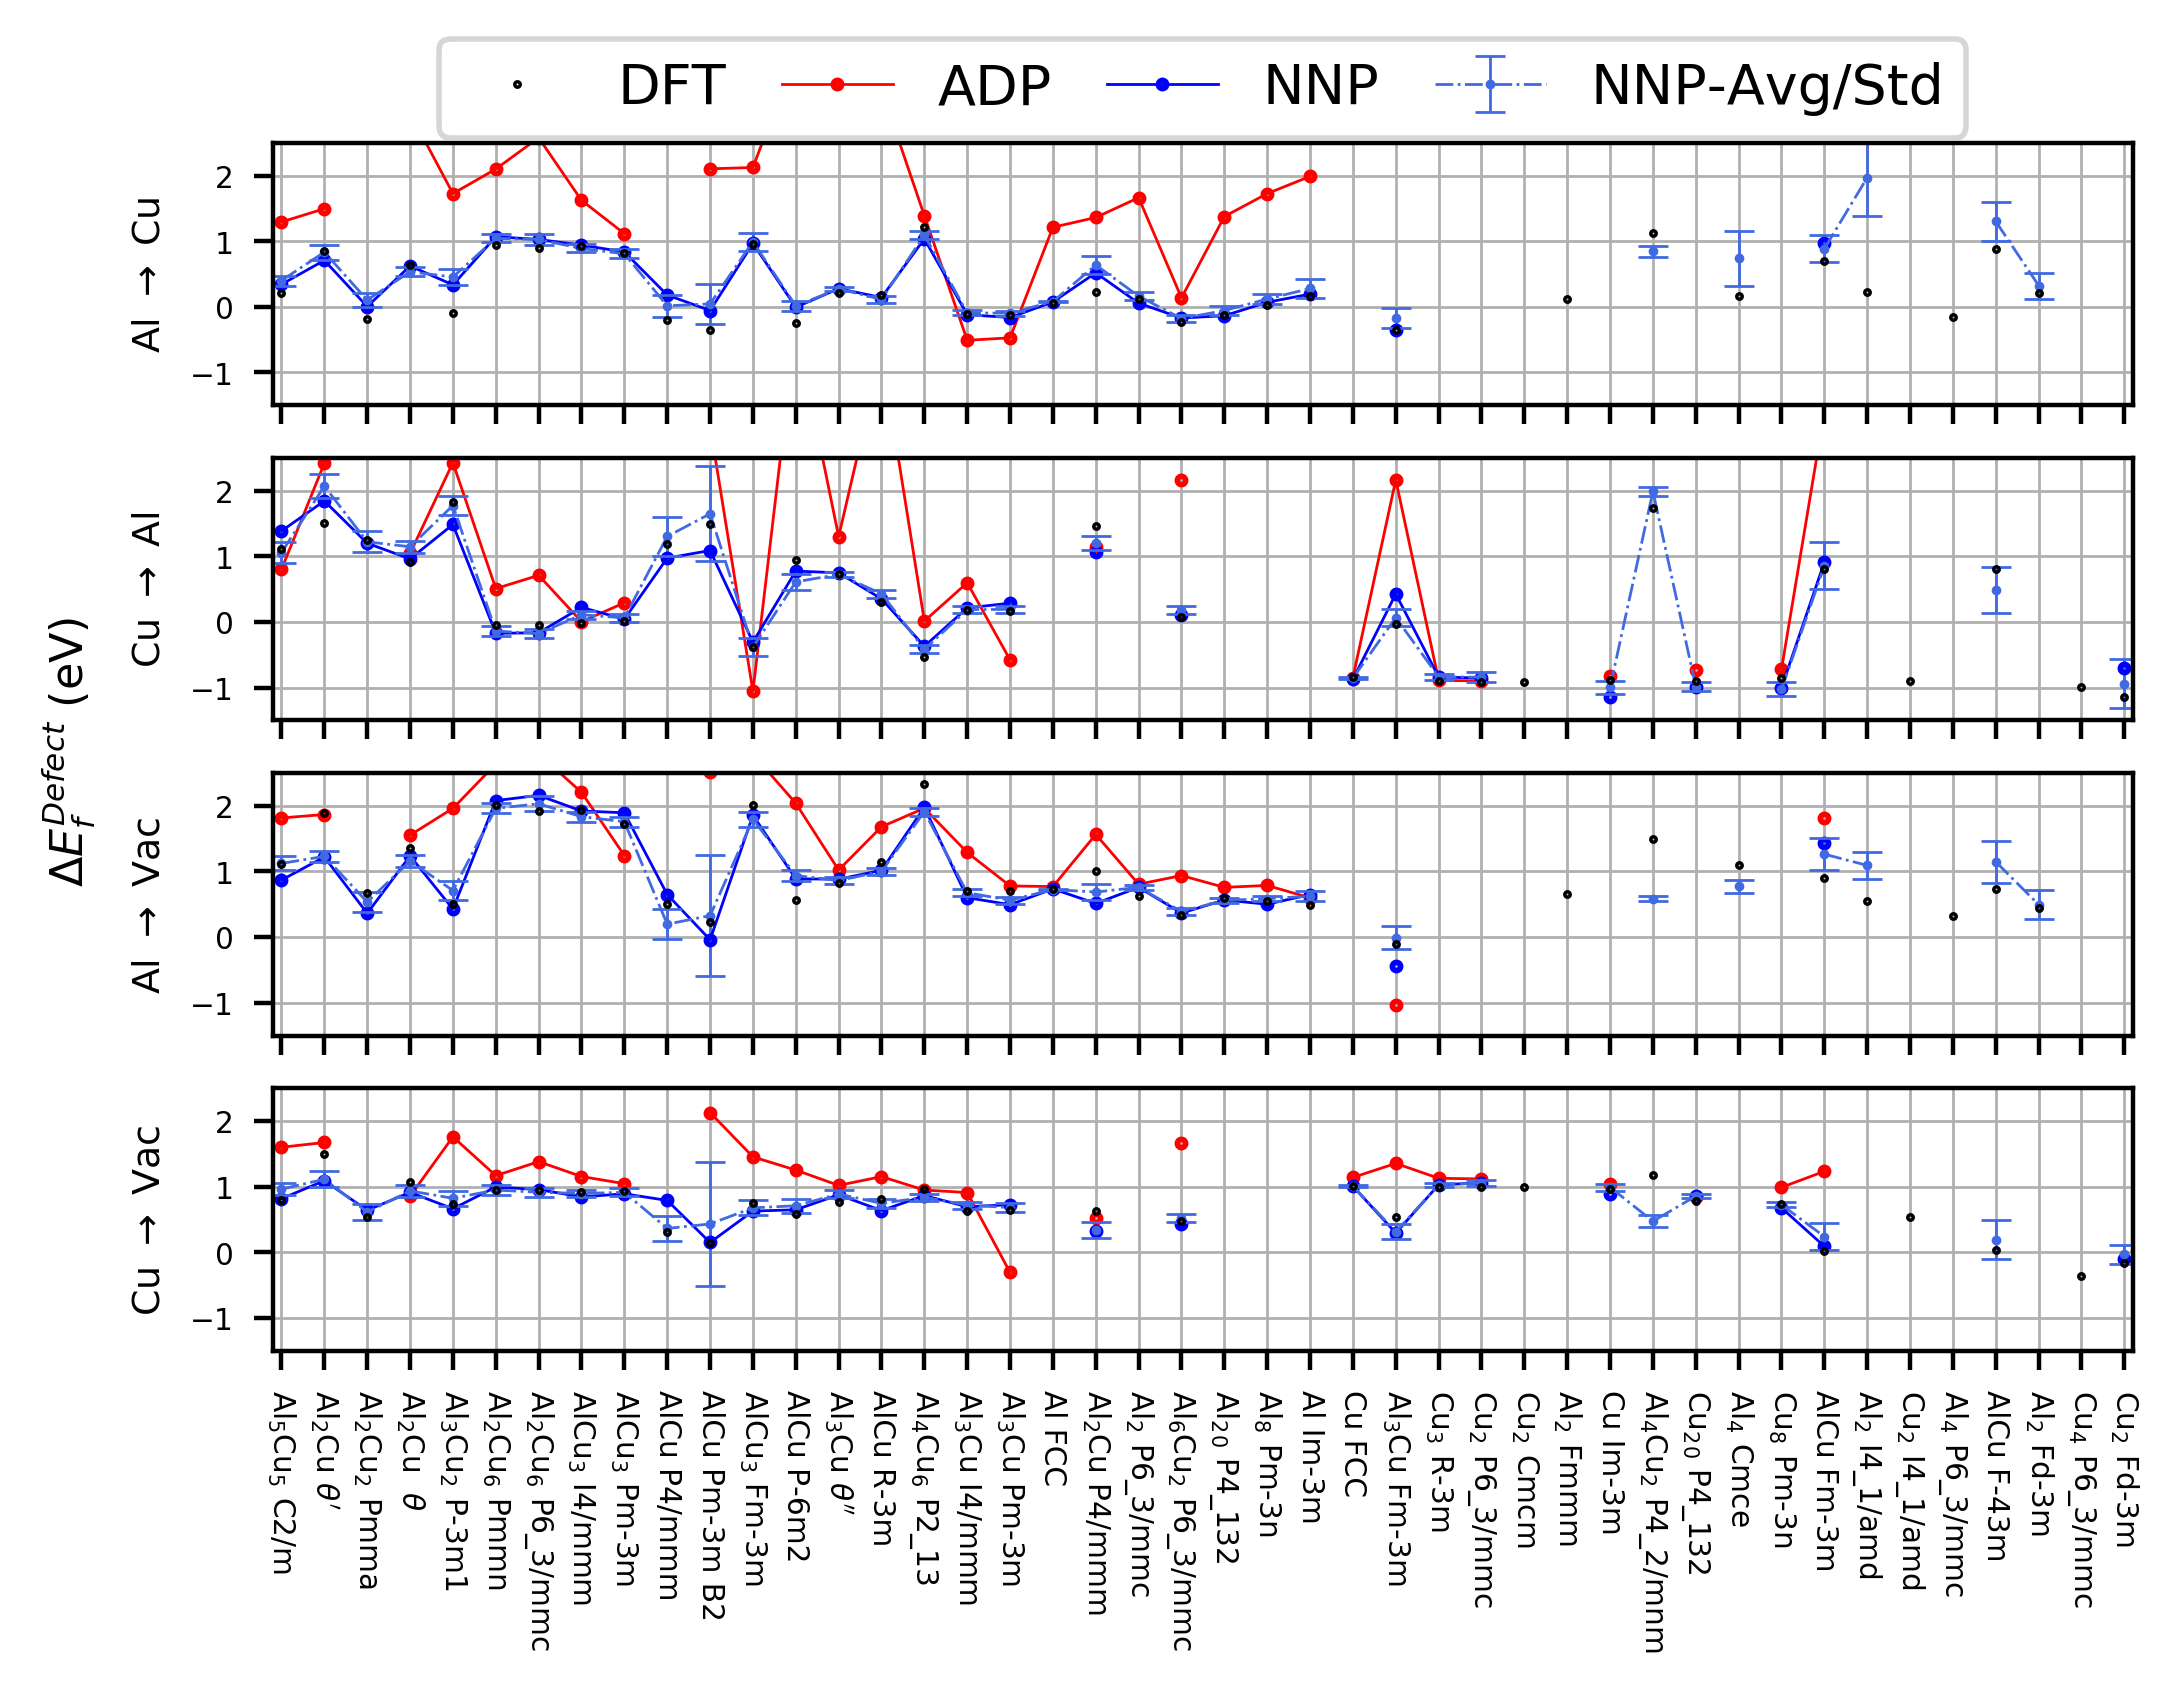
\includegraphics[width=1.2\textwidth,center]{figures/antisite_vacancies.png}%
\caption{DFT antisite formation energy vs. ADP/NNP antisite formation energy.
These structures were not included in the training set.}%
\label{fig:antisite_plot}
\end{figure}

\newpage
\bibliographystyle{unsrt}  
\bibliography{references}  %%% Remove comment to use the external .bib file (using bibtex).
%%% and comment out the ``thebibliography'' section.

\newpage
\appendix
\section{Supplementary}
\begin{figure}[H]%
\centering%
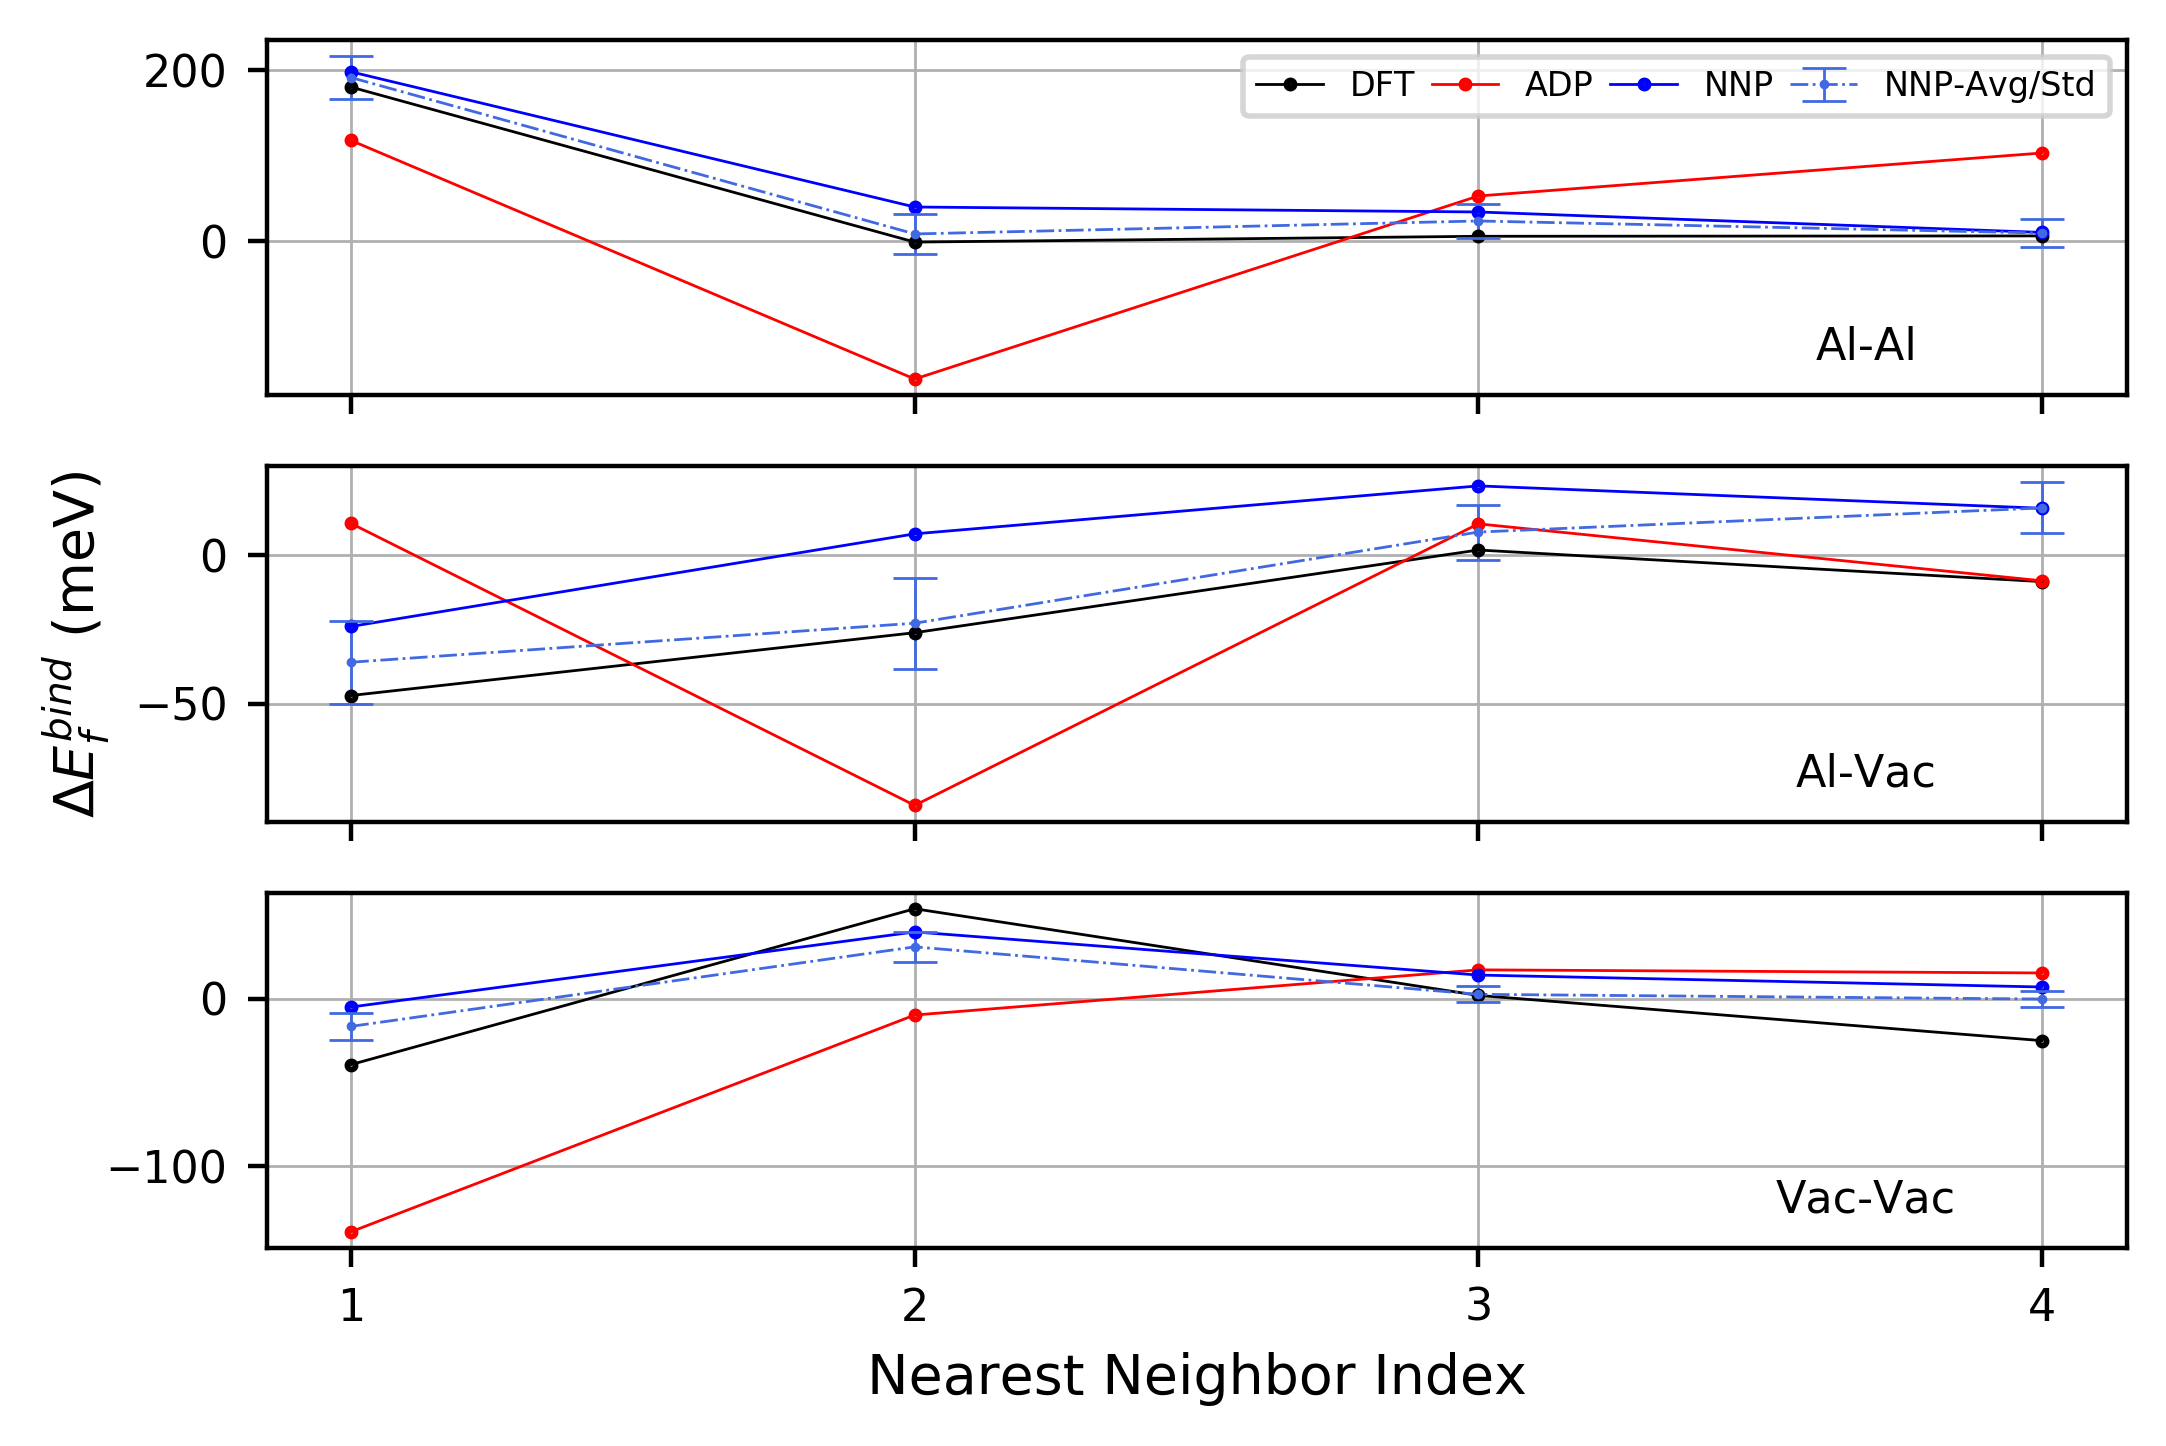
\includegraphics[width=1.2\textwidth,center]{./figures/solsol_in_cu.png}%
\caption{Neighbor index vs. binding energy $E_{bind}$ for Al-Al, Al-Vac and Vac-Vac in Cu matrix.}%
\label{fig:solsol_in_cu}
\end{figure}


\begin{figure}[H]%
\centering%
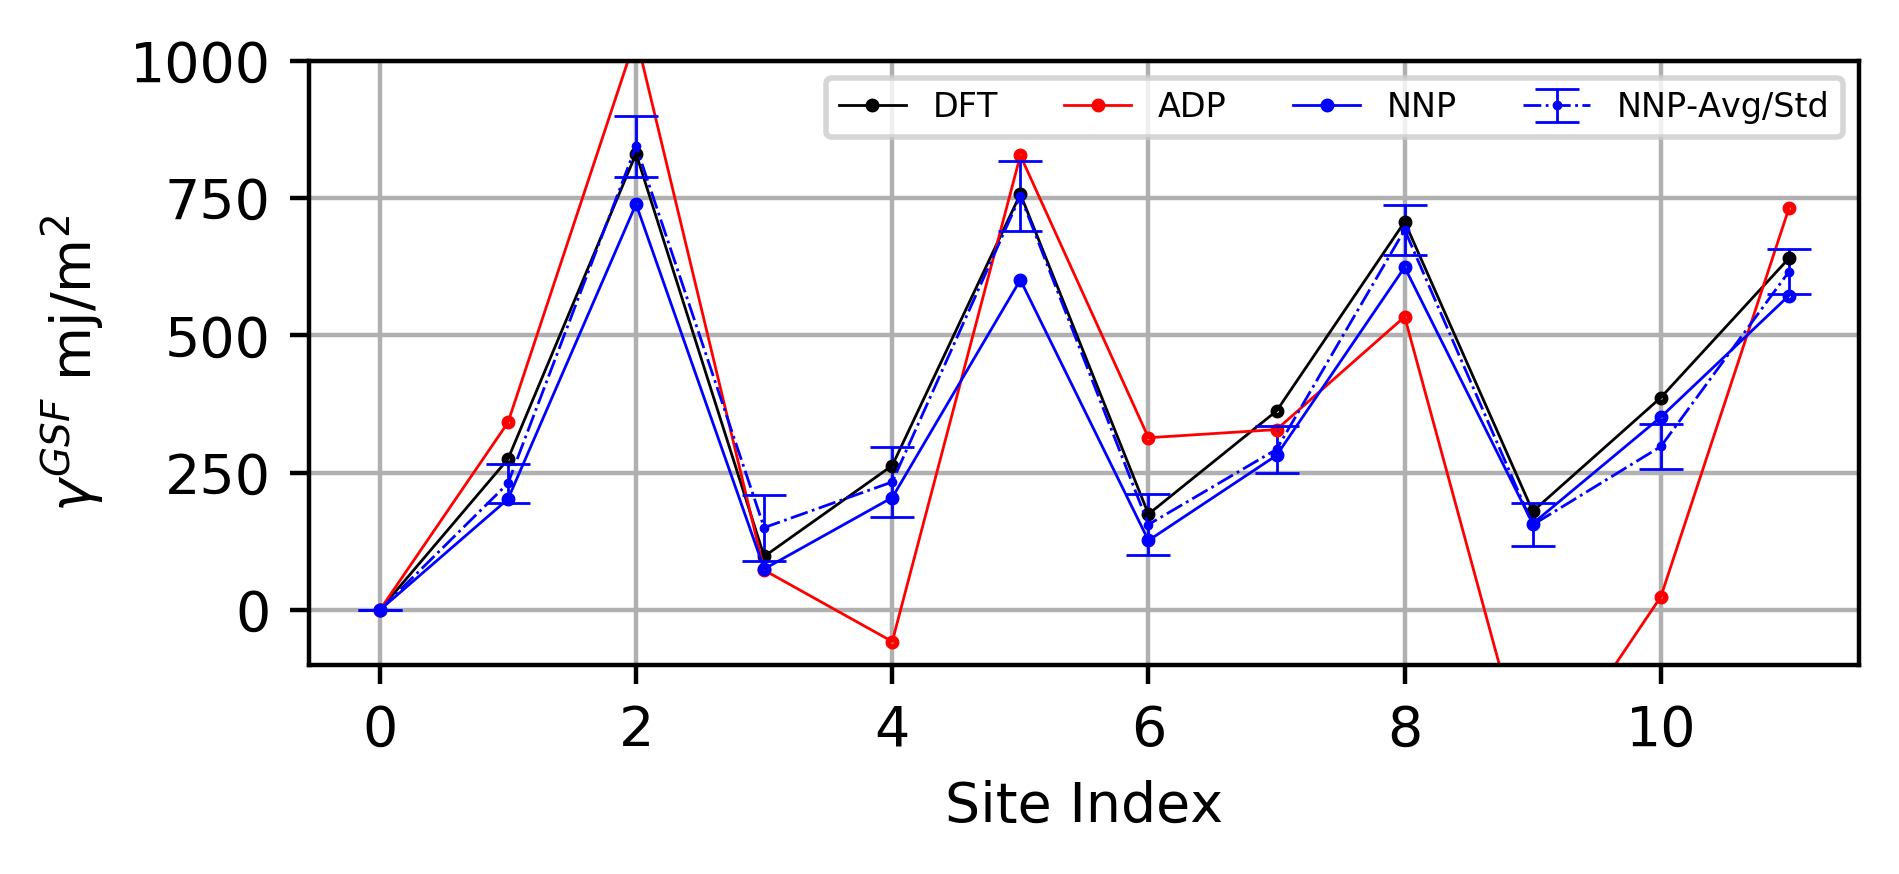
\includegraphics[width=540px]{./figures/NOTINOQMD_00002-GSF_111.png}%
\caption{GSF energy for key sites on the 111 surface of  $\theta''$.These sites are not included in the  training set for NNP}%
\end{figure}

\begin{figure}[H]%
\centering%
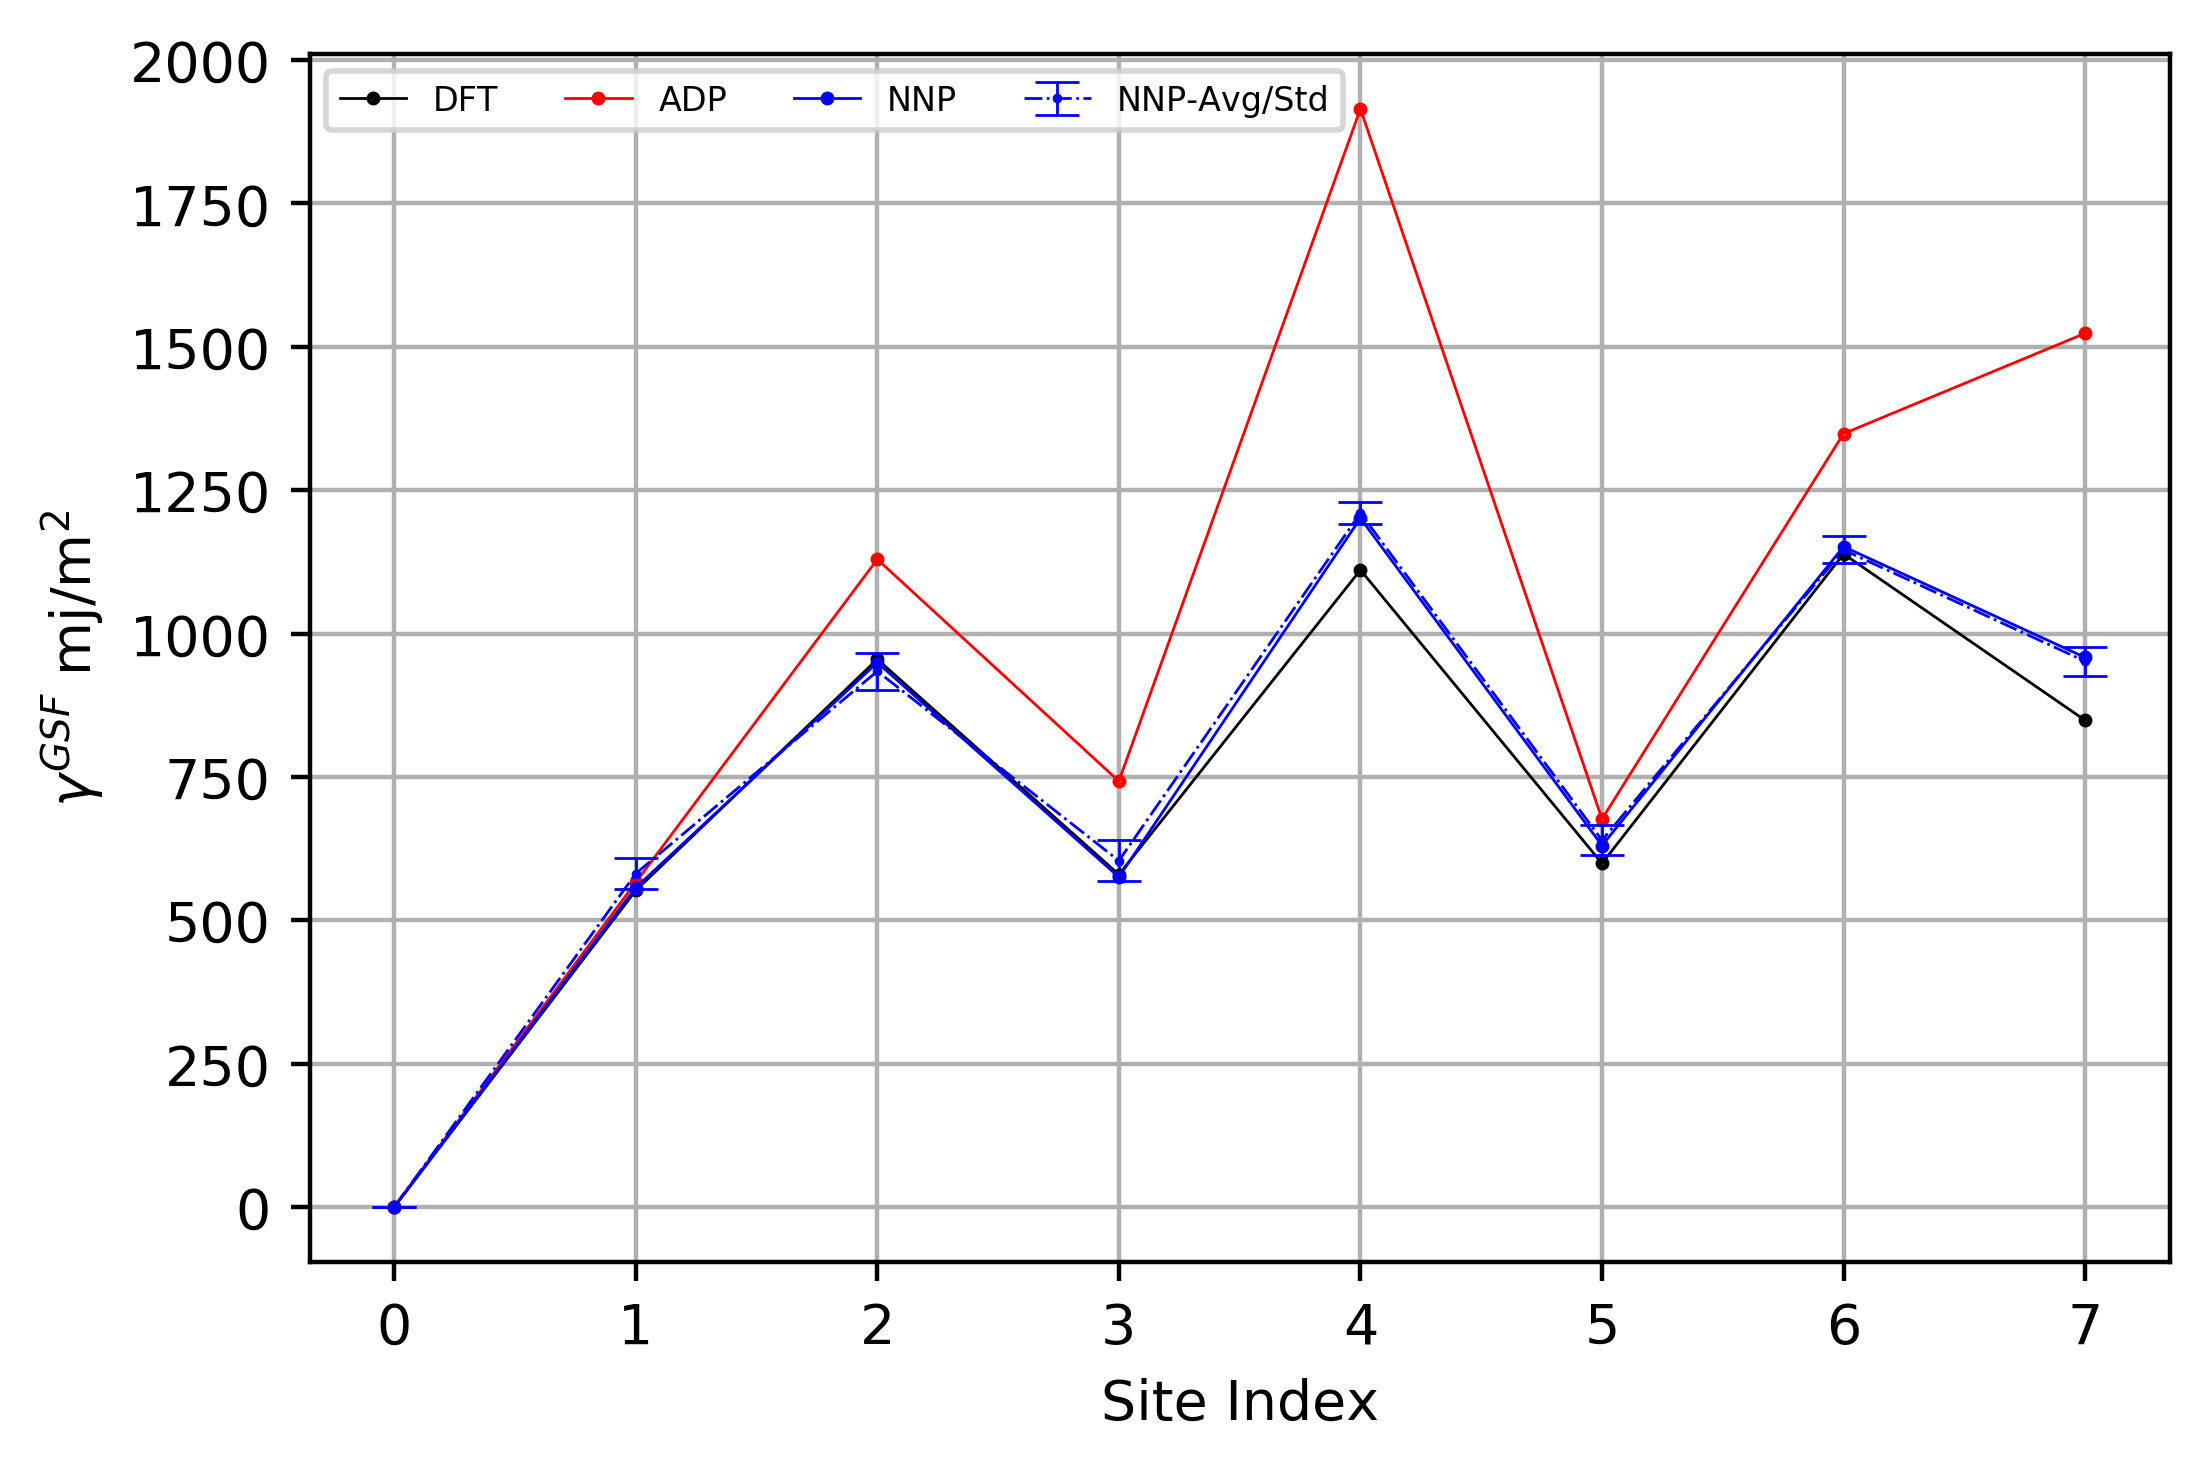
\includegraphics[width=540px]{./figures/NOTINOQMD_00001-GSF_0m11.png}%
\caption{GSF energy for key sites on the 0-11 surface of  $\theta$. These sites are included in the training set for NNP}%
\end{figure}


\begin{tabular}{l|lll|lll}%
\hline%
Structure&\multicolumn{3}{c}{FCC Al}&\multicolumn{3}{c}{FCC Cu}\\%
Method&DFT&NNP&ADP&DFT&NNP&ADP\\%
\hline%
a ($\AA$)&4.04&4.047&4.05&3.625&3.627&3.615\\%
vol/atom ($\AA^3$)&16.48&16.58&16.61&11.9&11.93&11.81\\%
G (GPa)&30.7&33.0&29.6&59.4&62.6&55.3\\%
K (GPa)&78.2&77.2&78.5&143.9&146.3&138.9\\%
$C_{11}$ (GPa)&112.5&110.6&113.5&180.3&182.4&170.4\\%
$C_{21}$ (GPa)&61.0&60.5&61.1&125.7&128.2&123.2\\%
$C_{44}$ (GPa)&34.0&38.2&31.9&80.8&86.3&76.5\\%
\hline%
\end{tabular}%
\newline%
\newline%
\newline%
\newline%

\begin{tabular}{l|ccc|ccc|ccc}%
\hline%
Structure&\multicolumn{3}{c}{Al$_2$Cu  $\theta$}&\multicolumn{3}{c}{Al$_2$Cu $\theta'$}&\multicolumn{3}{c}{Al$_3$Cu $\theta''$}\\%
Method&DFT&NNP&ADP&DFT&NNP&ADP&DFT&NNP&ADP\\%
\hline%
a ($\AA$)&4.869&4.917&4.862&4.087&4.095&3.994&2.804&2.792&2.784\\%
b ($\AA$)&4.926&4.929&4.862&4.087&4.095&3.994&2.804&2.792&2.784\\%
c ($\AA$)&4.926&4.929&4.862&4.087&4.095&3.994&7.65&7.65&7.586\\%
$\alpha$&75.9&75.6&75.2&60.0&60.0&60.0&90.0&90.0&90.0\\%
$\beta$&60.4&60.1&75.2&60.0&60.0&60.0&90.0&90.0&90.0\\%
$\gamma$&60.4&60.1&60.6&60.0&60.0&60.0&90.0&90.0&90.0\\%
vol/atom ($\AA^3$)&14.88&14.95&14.41&16.09&16.18&15.02&15.04&14.9&14.69\\%
$\Delta$$H^{comp}$ (meV/atom)&{-}161.6&{-}162.9&{-}189.8&{-}184.0&{-}184.0&{-}202.6&{-}94.2&{-}94.8&{-}128.8\\%
G (GPa)&42.3&39.3&57.5&56.6&56.5&44.1&48.8&40.6&32.6\\%
K (GPa)&100.8&115.7&154.5&97.0&96.8&138.6&94.3&89.5&84.9\\%
$C_{11}$ (GPa)&170.4&167.8&199.5&158.7&160.4&192.4&160.5&148.6&115.4\\%
$C_{22}$ (GPa)&170.4&167.8&199.5&158.7&160.4&192.4&160.5&148.6&115.4\\%
$C_{33}$ (GPa)&174.8&180.4&278.2&158.7&160.4&192.4&181.8&154.1&142.0\\%
$C_{44}$ (GPa)&28.8&37.0&80.0&63.5&62.3&46.5&45.8&32.4&38.2\\%
$C_{55}$ (GPa)&28.8&37.0&80.0&63.5&62.3&46.5&45.8&32.4&38.2\\%
$C_{66}$ (GPa)&47.5&38.1&21.0&63.5&62.3&46.5&42.2&46.6&27.4\\%
$C_{21}$ (GPa)&73.7&104.2&99.3&66.2&64.9&111.6&70.9&61.6&48.0\\%
$C_{31}$ (GPa)&61.1&79.2&128.7&66.2&64.9&111.6&51.1&57.6&73.8\\%
$C_{32}$ (GPa)&61.1&79.2&128.7&66.2&64.9&111.6&51.1&57.6&73.8\\%
\hline%
\end{tabular}%



\end{document}
